% SC6131 Capstone Final Report — Nanyang Technological University
% Student: Yiqun Xu (Franz), G2509092H
% Build: latexmk -pdf main.tex   (or: pdflatex main && pdflatex main)
\documentclass[11pt,a4paper]{article}

% ---------------------------------------------------------------------------
% Packages
% ---------------------------------------------------------------------------
\usepackage[T1]{fontenc}
\usepackage[utf8]{inputenc}
\usepackage{lmodern}
\usepackage{microtype}
\usepackage[margin=25mm]{geometry}
\usepackage{setspace}
\usepackage{amsmath,amssymb}
\usepackage{booktabs}
\usepackage{array}
\usepackage{tabularx}
\usepackage{multirow}
\usepackage{graphicx}
\usepackage{xcolor}
\usepackage{enumitem}
\usepackage{caption}
\usepackage{listings}
\usepackage{tikz}
\usetikzlibrary{arrows.meta,positioning,fit,calc,shapes.misc}
\usepackage{float}
\usepackage[hidelinks,breaklinks]{hyperref}
\usepackage{url}

% ---------------------------------------------------------------------------
% Typography and layout
% ---------------------------------------------------------------------------
\onehalfspacing
\emergencystretch=2em
\setlist{noitemsep,topsep=3pt}
\urlstyle{tt}
\captionsetup{font=small,labelfont=bf}
\setcounter{tocdepth}{2}
\setcounter{secnumdepth}{3}

% Listings: monospace code with light framing, JSON/YAML/shell friendly.
\definecolor{codebg}{RGB}{247,247,249}
\definecolor{codeframe}{RGB}{210,210,215}
\definecolor{codecomment}{RGB}{110,110,120}
\lstset{
  basicstyle=\ttfamily\small,
  backgroundcolor=\color{codebg},
  frame=single,
  rulecolor=\color{codeframe},
  framerule=0.4pt,
  xleftmargin=6pt,
  xrightmargin=6pt,
  breaklines=true,
  breakatwhitespace=false,
  columns=fullflexible,
  keepspaces=true,
  showstringspaces=false,
  commentstyle=\color{codecomment}\itshape,
  tabsize=2,
  upquote=true,
  literate={≤}{{$\leq$}}1 {≥}{{$\geq$}}1 {—}{{---}}1 {–}{{--}}1 {→}{{$\rightarrow$}}1 {≈}{{$\approx$}}1 {×}{{$\times$}}1,
}
\lstdefinelanguage{yaml}{
  keywords={true,false,null},
  sensitive=false,
  comment=[l]{\#},
}
\lstdefinelanguage{json}{
  string=[b]",
  comment=[l]{//},
  literate=
    *{0}{{{\color{black}0}}}{1}
     {1}{{{\color{black}1}}}{1}
     {2}{{{\color{black}2}}}{1}
     {3}{{{\color{black}3}}}{1}
     {4}{{{\color{black}4}}}{1}
     {5}{{{\color{black}5}}}{1}
     {6}{{{\color{black}6}}}{1}
     {7}{{{\color{black}7}}}{1}
     {8}{{{\color{black}8}}}{1}
     {9}{{{\color{black}9}}}{1}
     {:}{{{\color{black}{:}}}}{1}
     {,}{{{\color{black}{,}}}}{1},
}

% ---------------------------------------------------------------------------
% Metadata macros (single source of truth for the fixed facts)
% ---------------------------------------------------------------------------
\newcommand{\ReportTitle}{Paid Attention for Personal AI Agents:\\Notification Coalescing, Attention Metering and Prepaid Postage in the Trusted Agents Protocol}
\newcommand{\StudentName}{Yiqun Xu (Franz)}
\newcommand{\StudentId}{G2509092H}
\newcommand{\StudentEmail}{yxu064@e.ntu.edu.sg}
\newcommand{\Programme}{MSc in Blockchain (MSBT), November 2025 Intake}
\newcommand{\CourseCode}{SC6131 Capstone Project}
\newcommand{\Partner}{Taiko}
\newcommand{\Mentor}{Daniel Wang (dan@taiko.xyz)}
\newcommand{\Supervisor}{Alvin Song}
\newcommand{\Teammate}{Zhang Hanyu (Jack Zhang)}
\newcommand{\DueDate}{18 October 2026, 23:59 SGT}
\newcommand{\RepoUrl}{https://github.com/IcantFind-a-username/trusted-agents}
\newcommand{\PrUrl}{https://github.com/IcantFind-a-username/trusted-agents/pull/1}
\newcommand{\Branch}{feat/phase1-notification-coalescing}

% Inline code helper that survives line breaks in narrow columns.
\newcommand{\code}[1]{\texttt{#1}}

\hypersetup{
  pdftitle={SC6131 Capstone Final Report — Paid Attention for Personal AI Agents},
  pdfauthor={Yiqun Xu},
  pdfsubject={NTU MSBT SC6131 Capstone Final Report},
}

\begin{document}

% ---------------------------------------------------------------------------
% Title page
% ---------------------------------------------------------------------------
\begin{titlepage}
\centering
\vspace*{10mm}

{\large\textsc{Nanyang Technological University}\par}
{\normalsize College of Computing and Data Science\par}
\vspace{2mm}
{\normalsize \Programme\par}

\vspace{18mm}

{\large\textbf{\CourseCode}\par}
{\normalsize Final Report\par}

\vspace{14mm}

{\LARGE\bfseries\setstretch{1.15} \ReportTitle\par}

\vspace{20mm}

\begin{tabular}{@{}r@{\hspace{1.2em}}l@{}}
\textbf{Student}      & \StudentName \\
\textbf{Matric.\ No.} & \StudentId \\
\textbf{E-mail}       & \href{mailto:\StudentEmail}{\StudentEmail} \\[6pt]
\textbf{Industry Partner} & \Partner \\
\textbf{Industry Mentor}  & \Mentor \\
\textbf{Academic Supervisor} & \Supervisor \\
\textbf{Project Teammate}    & \Teammate \\[6pt]
\textbf{Submission Deadline} & \DueDate \\
\end{tabular}

\vfill

\begin{minipage}{0.86\textwidth}
\small
\textbf{Artefact.} The implementation described in this report is the branch
\code{\Branch} of the repository \url{\RepoUrl}, submitted as pull request~\#1:
\url{\PrUrl}. The evaluation artefacts (\path{evaluation/results.md} and the
benchmark scripts) were contributed by the project teammate and merged into the same
branch as pull request~\#2 (merge commit \code{0330091}).

\medskip
\textbf{Declaration.} This is an individual report. The division of work between the
two team members is stated explicitly in Section~\ref{sec:project-management}. All
quantitative results are reproduced from the teammate's evaluation record without
alteration and are attributed accordingly.
\end{minipage}

\vspace{8mm}
\end{titlepage}


\pagenumbering{roman}
\section*{Abstract}
\addcontentsline{toc}{section}{Abstract}

Personal AI agents that talk to one another over an open messaging network expose a
resource that existing anti-spam mechanisms do not price: the receiving agent's
large-language-model (LLM) context. Every inbound peer message is eventually rendered
into the receiver's prompt, where it costs tokens, and some messages additionally wake
an idle agent. Neither cost is borne by the sender, and a flood of low-value chatter can
bury a genuinely important event---such as a pending transfer approval---below a rendering
cap.

This report describes the design and implementation of a paid-attention layer for the
Trusted Agents Protocol (TAP), a local-first protocol in which agents hold ERC-8004
identities, connect through signed invites, and exchange JSON-RPC messages over XMTP. The
work was carried out with Taiko as industry partner. The initial project plan, recorded in
the first progress journal, was to build a standalone ``Tack-like'' TypeScript service
that charged for message delivery through x402 payments on Taiko Alethia. That plan was
deliberately revised: because the scarce resource is the receiver's attention rather than
storage or bandwidth at a relay, the meter belongs in the receiver's own TAP daemon, where
the cost is actually incurred and where authenticated peer identity and permission grants
already exist. The result is a TAP-native design that retains the x402 idea---a
machine-readable ``payment required'' response carrying a quote---but carries it over XMTP
as JSON-RPC error \code{-32050}.

The implementation, contributed by the author, proceeds in dependency order.
(1)~Notification coalescing and escalation-first rendering reduce injected context and
guarantee that escalations are never displaced by chatter. (2)~A file-backed attention
ledger measures, per peer and per day, the notification lines rendered, the estimated
tokens injected, the escalations surfaced and the events suppressed. (3)~Optional
attention pricing advertises per-tier prices in the agent's registration file and, when
enforcement is enabled (default off), rejects un-granted messages with a quote.
(4)~Prepaid postage lets a sender pay once on-chain, receive a signed credit certificate,
and then attach stamps to many messages; a strictly increasing sequence number and a
single-writer ledger make stamps replay- and double-spend-resistant. (5)~Priority stamps
buy an escalation and, in OpenClaw, an immediate wake-up, while a
\code{notificationsPerWeek} grant constraint folds an over-quota grant holder's chatter
into one summary line without ever dropping a message.

The evaluation, designed and executed by the project teammate, shows that under floods
of 50 to 1000 messages the coalescing pipeline reduces estimated injected tokens by
79.3--79.7\% relative to the legacy FIFO renderer while keeping the escalation visible in
every case, that the legacy pipeline hides the escalation at 50 messages and above, and that
a 0.002~USDC prepaid credit at 0.001~USDC per message admits exactly two messages before
the third is rejected with \code{insufficient\_credit}. The report closes with an honest
account of the limitations: token counts are a \code{chars/4} approximation, the
payment-verification hook accepts claimed transactions unless a host supplies chain
access, and the priority/quota experiment could not be executed locally because the OWS
native binary is unavailable on Windows.

\medskip
\noindent\textbf{Keywords:} AI agents, attention economics, anti-spam, prepaid credits,
x402, XMTP, ERC-8004, Taiko, local-first systems.

\clearpage
\tableofcontents
\clearpage
\listoftables
\listoffigures
\clearpage

\pagenumbering{arabic}
\section{Introduction}
\label{sec:introduction}

\subsection{Context}

The Trusted Agents Protocol (TAP) is an open-source, local-first protocol stack that lets
personal AI agents---an OpenClaw or Hermes assistant run by one person---find, verify and
message the agents run by people they already know~\cite{tap-repo}. Each agent holds an
on-chain identity as an ERC-8004 token~\cite{erc8004}, publishes a registration file
describing its messaging endpoint, connects to peers through signed invitation links, and
exchanges JSON-RPC~2.0 payloads over the XMTP messaging network~\cite{xmtp}. Owners
control what a peer may ask for through \emph{directional permission grants}, for example
``may request up to 10~USDC per week''. TAP is explicitly built for trust between known
humans mediated through their agents, not for an open marketplace.

Taiko, the industry partner for this capstone, operates an Ethereum-based rollup
(Taiko Alethia) and had already integrated with TAP at the identity layer: agents can
register on Taiko (\code{eip155:167000}) and can upload their registration file through
\emph{Tack} (\code{tack.taiko.xyz}), Taiko's x402-metered IPFS upload
service~\cite{x402}. The project brief extended this from paid storage to a broader notion
of paid interaction between agents.

\subsection{Problem}

Once two agents are connected, TAP as of April~2026 delivered every peer message into the
receiving agent's context without any notion of cost. This creates three concrete
problems, all observed in the codebase before this work:

\begin{enumerate}
  \item \textbf{Unmetered attention.} A peer message costs the \emph{receiver} LLM tokens on
        every prompt into which it is rendered, and in streaming hosts it can wake an idle
        agent. The sender pays nothing. This is structurally the same externality that
        made e-mail spam economically rational~\cite{dwork-naor,hashcash}.
  \item \textbf{Buried escalations.} The notification block injected into the agent's prompt
        was rendered first-in-first-out with a hard cap of twenty lines. A burst of chatter
        arriving before a transfer-approval request pushed the request into an opaque
        ``$N$ more omitted'' footer. The one line the operator most needed to see was the
        one most likely to be hidden.
  \item \textbf{No vocabulary for pricing.} Even if a receiver wanted to charge for attention,
        the protocol had no way to advertise a price, no error that a sender could interpret
        as ``payment required'', and no unit in which attention could be measured or billed.
\end{enumerate}

\subsection{Objectives}

The capstone set out to make LLM attention a first-class, measurable and optionally
prepaid resource on top of TAP's existing invite-and-grant trust baseline. Concretely:

\begin{enumerate}[label=O\arabic*.]
  \item Reduce the context a message flood injects into the receiver's prompt, and
        guarantee that escalations are always rendered.
  \item Measure attention spend per peer so that pricing decisions rest on data.
  \item Let an agent advertise attention prices and reject un-granted, unpaid messages
        with a machine-readable quote, without changing the behaviour of any agent that
        does not opt in.
  \item Provide prepaid postage so that a sender pays once and spends many times, with
        replay and double-spend protection.
  \item Let a sender pay for an escalation (a ``priority'' message) and let a receiver
        meter the free tier of a grant holder through a weekly notification quota.
  \item Validate the mechanisms with a reproducible evaluation.
\end{enumerate}

\subsection{A change of approach, stated up front}

The first progress journal proposed to meet these objectives with a standalone
TypeScript service modelled on Tack: senders would pay per message through x402 on Taiko
Alethia, and the service would gate delivery. The implemented system does not do this.
Section~\ref{sec:design-pivot} sets out why: the scarce resource is the receiver's
attention, which only the receiver's own daemon can observe and account for; TAP already
supplies authenticated peer identity and grants that a standalone service would have to
duplicate; and the upstream TAP maintainers' research note for the messaging layer argued for keeping
chain RPC out of the hot path in favour of prepaid credits~\cite{tap-research-note}. The
change was a design decision taken with the full time budget available, not a fallback.
The x402 idea survives in the implemented system as a ``402 over XMTP'': a JSON-RPC
\code{-32050} error whose \code{data} carries the same price list the agent publishes on
chain.

\subsection{Contributions and division of work}

This is an individual report on a two-person project. The author (Yiqun Xu) designed and
implemented the entire paid-attention layer described in
Sections~\ref{sec:design}--\ref{sec:implementation}: 23~implementation commits on the
branch \path{feat/phase1-notification-coalescing}, roughly 8{,}200 added lines across
91~files, including a new workspace package \code{@trustedagents/app-postage}, mock
end-to-end test phases~6--8, and the accompanying documentation in the TAP skill file. The
teammate (Zhang Hanyu) led the earlier design exploration and owned the evaluation:
the benchmark scripts and \path{evaluation/results.md} merged as pull request~\#2. All
figures in Section~\ref{sec:evaluation} are his and are reproduced exactly.
Section~\ref{sec:project-management} gives the full account, including the fact that the
industry mentor has been unreachable since late August~2026 and that the final design
therefore carries no mentor sign-off.

\subsection{Report structure}

Section~\ref{sec:background} introduces TAP, the surrounding standards and the related
work on attention pricing. Section~\ref{sec:requirements} states the requirements and the
threat model. Section~\ref{sec:design} presents the design and its rationale, including
the pivot away from a standalone service. Section~\ref{sec:implementation} describes the
implementation. Section~\ref{sec:evaluation} reports the evaluation.
Section~\ref{sec:discussion} discusses limitations and security considerations.
Section~\ref{sec:project-management} covers project management and the division of
labour. Section~\ref{sec:conclusion} concludes with future work. Appendices reproduce
the operator-facing configuration, the wire formats and the commit log.

\section{Background and Related Work}
\label{sec:background}

\subsection{The Trusted Agents Protocol}

TAP is organised as a small monorepo of TypeScript packages with a strict dependency
direction~\cite{tap-repo}. \code{core} owns the wire protocol, identity resolution, the
XMTP transport, the trust store (contacts and grants), conversation logging and the
request journal. Host adapters compose \code{core} without re-implementing it: the
\code{tap} command-line interface, \code{tapd} (a long-lived daemon that holds the single
XMTP client for one identity and exposes a local HTTP API), the OpenClaw Gateway plugin and
the Hermes integration. The repository's own guidance summarises the discipline as
``thin plugin, fat CLI'': a host may only expose what requires a live transport
connection.

Three properties of the pre-existing system shaped the present work.

\paragraph{Identity and trust are already authenticated.}
An agent's identity is an ERC-8004 token~\cite{erc8004}; its \code{tokenURI} points to a
registration file that names the agent's XMTP endpoint address, and \code{ownerOf}
identifies its owner. A peer is admitted only after a signed invite has been exchanged and
recorded as an \emph{active contact}; unknown senders are rejected at the transport
boundary. Grants are directional: the receiver records what it has granted to each peer
(\code{grantedByMe}) with a scope such as \code{message/send} or \code{transfer/request}
and optional constraints. Every signing operation---invites, EIP-7702 or ERC-4337
transactions, and now postage certificates---goes through an Open Wallet Service (OWS)
signing provider; the agent process never holds a raw private key.

\paragraph{Messages are JSON-RPC over XMTP.}
The canonical methods~\cite{jsonrpc} are \code{connection/request},
\code{connection/result} and \code{connection/revoke} for the handshake,
\code{permissions/update} for grants, \code{message/send} for chat, and
\code{action/request} with \code{action/result} for typed actions. Applications extend the
protocol by registering \emph{action types} (for example \code{transfer/request} or
\code{scheduling/propose}) with the app registry; a \emph{TAP app} is a package that
defines handlers for its action types and is installed from a manifest.

\paragraph{The daemon owns a notification pipeline.}
\code{tapd} classifies typed runtime events (\code{message.received},
\code{action.pending}, \code{connection.established}, \ldots) into
\code{TapNotification} records of type \code{info}, \code{escalation}, \code{auto-reply}
or \code{summary}, buffers them in an in-memory queue, and lets hosts drain the queue.
OpenClaw drains it in a \code{before\_prompt\_build} hook and injects a
\code{[TAP Notifications]} block into the agent's prompt; escalations additionally call
\code{requestHeartbeatNow()} to wake the agent. Hermes has no wake API and shows the block
on the next turn~\cite{tapd-spec}. Before this project, the queue was append-only and the
renderer emitted the first twenty lines in arrival order.

\subsection{Taiko, Tack and x402}

Taiko Alethia is a based rollup on Ethereum; TAP supports it as a registration chain
alongside Base~\cite{taiko}. x402 is an HTTP-native payment protocol that revives the
reserved \code{402 Payment Required} status: a server answers an unpaid request with a
machine-readable price, the client pays and retries with a payment proof, and a
facilitator verifies settlement~\cite{x402}. Tack is Taiko's x402-metered IPFS upload
service; TAP's \code{tap register --ipfs-provider tack} pays for the upload of the
registration file with USDC on Taiko. Tack therefore meters a resource located at the
service---storage---at the moment of the request. The question this capstone had to
answer was whether the same pattern was the right one for a resource located at the
receiving \emph{peer}.

\subsection{Attention as the scarce resource}

The observation that ``a wealth of information creates a poverty of attention'' is
Simon's~\cite{simon}. For LLM-hosted agents the observation is literal: an agent's working
memory is a bounded token window, each token in it has a monetary and latency cost, and an
idle agent that is woken pays a fixed cost per wake regardless of the message's value.
Attention here has three distinguishable prices---context (tokens per prompt), wake-ups
(interrupt cost), and the operator's time when an approval is requested---and a good
metering design should be able to separate them.

\subsection{Related work on pricing unsolicited messages}

\paragraph{Proof of work.} Dwork and Naor proposed that a sender attach a moderately hard
computation to each message so that bulk sending becomes expensive~\cite{dwork-naor};
Hashcash made the idea deployable~\cite{hashcash}, and memory-bound variants were
explored to equalise cost across hardware~\cite{abadi}. Laurie and Clayton showed that,
for e-mail, any work parameter cheap enough for legitimate senders is cheap enough for
spammers renting compromised machines~\cite{laurie-clayton}. In the present setting the
argument is stronger still: an agent that floods a peer is not necessarily malicious---it
may be a well-meaning agent with a verbose prompt---so the cost should be legible and
attributable, which computation is not and money is.

\paragraph{Rate-limited relays.} Waku's RLN-Relay attaches a zero-knowledge rate-limiting
nullifier to each message so that relays can slash a member who exceeds an epoch
quota~\cite{waku-rln}. This protects the \emph{relay}; it says nothing about whether a
message was worth reading. TAP's research note reached the same conclusion: relays should
verify cheap proofs and decrement balances, and never inspect payments in the hot
path~\cite{tap-research-note}.

\paragraph{Postage and paid delivery.} Sender-pays postage for e-mail was proposed and
piloted repeatedly and failed for reasons of coordination---no single party could compel
every mail server to honour a stamp. TAP's setting removes that obstacle: every message is
already pairwise, authenticated and delivered to a single daemon that the receiving owner
controls, so the receiver can unilaterally decide what a stamp buys.

\paragraph{Agent protocols.} Google's Agent-to-Agent protocol defines tasks, artefacts and
capability cards for agent interoperation~\cite{a2a} but does not price attention. TAP's
own research note surveyed A2A, XMTP, Waku, x402 and SIWX and recommended a two-step
payment model---on-chain payment converted once into credits, credits spent off-chain per
message~\cite{tap-research-note}. That recommendation is the direct ancestor of the
postage design in Section~\ref{sec:design}.

\section{Requirements and Threat Model}
\label{sec:requirements}

\subsection{Functional requirements}

The requirements below were derived from the three problems in
Section~\ref{sec:introduction} and refined against the codebase. Each is labelled so that
the design (Section~\ref{sec:design}) and the evaluation (Section~\ref{sec:evaluation})
can refer back to it.

\begin{description}[style=nextline,leftmargin=1.2em]
  \item[FR1 --- Bounded context under flood.] The notification block injected into the
        receiver's prompt must grow sub-linearly in the number of inbound messages from a
        peer; repeated events of the same kind from the same peer must collapse into one
        counted line.
  \item[FR2 --- Escalations always visible.] A pending approval, a failed connection or a
        paid priority message must be rendered regardless of how much chatter arrived
        before it, and regardless of the rendering cap.
  \item[FR3 --- Attention is measured.] The receiver must record, per peer and per day,
        how many notification lines were rendered on its behalf, how many estimated tokens
        those lines injected, how many escalations were surfaced and how many events were
        suppressed past the cap. The record must be readable without starting the
        transport.
  \item[FR4 --- Prices are discoverable.] An agent must be able to publish attention prices
        per tier in the same registration file that already publishes its endpoint, so that
        a sender can learn the cost before sending, and preview it with a dry run.
  \item[FR5 --- Enforcement is opt-in and machine-readable.] With enforcement enabled, an
        inbound \code{message/send} from a sender that holds no active \code{message/send}
        grant and carries no valid stamp must be rejected \emph{before} it reaches the
        conversation log or the notification pipeline, with a JSON-RPC error whose
        \code{data} carries the price list and, when applicable, the reason the stamp failed.
        With enforcement disabled (the default) behaviour must be unchanged.
  \item[FR6 --- Grants are free stamps.] A peer that holds a \code{message/send} grant is
        never charged for standard delivery; the social trust encoded in a grant takes
        precedence over the economic mechanism.
  \item[FR7 --- Pay once, spend many.] A sender must be able to prepay a credit at a receiver
        with one on-chain payment and then send many messages, each carrying a stamp that is
        debited off-chain; no chain RPC may occur in the per-message path.
  \item[FR8 --- Portable proof of credit.] The receiver must return a signed certificate
        that binds the credit to the payment transaction, the two agent identities and the
        amount, verifiable by the holder against the receiver's known agent address.
  \item[FR9 --- Paid wake-ups.] A stamp whose value meets the receiver's published
        \code{priority} price must cause the message to render as an escalation, with a
        longer excerpt, and to wake the agent where the host supports it---including when
        the sender is a grant holder.
  \item[FR10 --- Metered free tier.] A \code{message/send} grant may carry a
        \code{notificationsPerWeek} constraint. When the holder exceeds it, further ordinary
        notifications in the window fold into one summary line; the messages themselves are
        still delivered and logged. Escalations are never folded.
  \item[FR11 --- Host parity.] Every mechanism must behave identically whether the host
        is the CLI, \code{tapd}, the OpenClaw plugin or the Hermes plugin, because all of
        them render the same drained batch.
\end{description}

\subsection{Non-functional requirements}

\begin{description}[style=nextline,leftmargin=1.2em]
  \item[NFR1 --- Backward compatibility.] A peer running a pre-project TAP version must be
        able to message and be messaged by a post-project peer. Stamps ride in message
        metadata that older peers ignore; enforcement defaults to off.
  \item[NFR2 --- Crash safety.] The ledgers are written by exactly one process (the
        transport owner) using the repository's existing \code{tmp + rename} pattern, and
        every wire interaction that moves money must be idempotent across a crash between
        payment, debit, journal write and event emission.
  \item[NFR3 --- Never lose a message.] Quota folding and coalescing may compress
        \emph{notifications}; they must never discard a \emph{message}. Any enforcement path
        that cannot answer (missing ledger, missing contact) must fail open.
  \item[NFR4 --- No new trusted third party.] The design must not introduce a service that
        both peers must trust in addition to the chain and XMTP.
  \item[NFR5 --- Repository conventions.] ESM, named exports, Biome lint/format, strict
        TypeScript with \code{noUnusedLocals}; every new CLI command documented in the
        canonical skill file; both E2E suites updated for behavioural changes.
\end{description}

\subsection{Threat model}
\label{sec:threat-model}

The adversary is a \emph{connected} peer: an agent that has completed the invite handshake
and is an active contact, but that may be buggy, over-eager or hostile. Unknown senders are
already rejected by the transport and are out of scope. The adversary can send arbitrary
\code{message/send} and \code{action/request} payloads at any rate, can replay its own
earlier messages, can present arbitrary stamps and can claim arbitrary transaction
hashes in a top-up. It cannot forge another agent's XMTP identity or OWS signatures. The
assets to protect are the receiver's LLM context, the receiver's wake budget, the
integrity of the postage ledger (no double spend, no minting) and the receiver's signing
key (no signing amplification). Section~\ref{sec:security} maps each threat to a
mitigation.

\section{Design}
\label{sec:design}

This section is the core of the report. It first explains why the architecture proposed
in the first progress journal was replaced (\S\ref{sec:design-pivot}), then states the
design principles that the replacement follows (\S\ref{sec:design-principles}), and
finally presents each mechanism with its rationale
(\S\ref{sec:design-coalescing}--\S\ref{sec:design-priority}).

\subsection{Where should the meter live?}
\label{sec:design-pivot}

\paragraph{The Journal-1 proposal.}
The first progress journal framed the project as ``Postage: paid attention'' and proposed
a standalone TypeScript service in the mould of Tack. A sender wishing to reach a receiver
would call the service, receive an x402 \code{402 Payment Required} with a price, pay in
USDC on Taiko Alethia, and retry; the service would then relay or release the message.
The proposal had real merits: it reused a payment flow the partner already operated, it
put Taiko in the per-message path, and it could be built without modifying TAP.

\paragraph{Why it was set aside.}
Working through the design against the codebase exposed four objections, any one of
which would have been sufficient.

\begin{enumerate}
  \item \textbf{It meters the wrong resource in the wrong place.} Tack prices bytes stored
        at Tack. The resource this project is about is the \emph{receiver's} LLM attention,
        and only the receiver's daemon knows what a message actually cost: whether it was
        rendered at all, into how many lines, whether it coalesced with earlier lines, whether
        it triggered a wake-up, whether it was suppressed past the cap. A service in front
        of the receiver can count messages or bytes; it cannot count attention. Pricing
        attention from outside the receiver would be pricing a proxy.
  \item \textbf{It duplicates a trust layer TAP already has.} TAP admits a sender only
        after an ERC-8004 identity has been resolved and a signed invite exchanged, and it
        already records per-peer grants. A standalone service would need its own account
        model, its own authentication of both parties and its own mapping from payer to
        recipient, all of which would have to be kept consistent with the trust store inside
        each daemon. It would also be a new party that both peers must trust with
        message-flow metadata, contradicting TAP's local-first design and NFR4.
  \item \textbf{It puts chain settlement in the hot path.} A per-message x402 payment means a
        transaction, or at least a facilitator round-trip, per message. The upstream TAP
        maintainers' research note for the messaging layer states the opposite requirement: ``Relays only
        need to verify the proof and decrement balance. No chain RPC is needed in the hot
        path''~\cite{tap-research-note}. The economically sound shape is one payment
        converted into many cheap spends.
  \item \textbf{It cannot compose with grants.} A friend who has been granted
        \code{message/send} should never pay; a stranger should. Only the receiver knows who
        holds a grant. Enforcing payment outside the receiver would either charge friends or
        require the receiver to publish its grant table to the service.
\end{enumerate}

\paragraph{The decision.}
Postage was therefore built \emph{into} TAP, at the receiver, as an extension of the
daemon that already renders notifications. Figure~\ref{fig:pivot} contrasts the two
shapes. What was kept from the x402 model is its most useful idea: an unpaid request is
answered not with silence but with a machine-readable quote. In the implemented system
that quote travels as JSON-RPC error \code{-32050} (\code{ATTENTION\_PAYMENT\_REQUIRED})
over XMTP, and the CLI and daemon surface it to local callers as HTTP \code{402}. What was
kept from the partner relationship is the settlement leg: a postage top-up is an on-chain
USDC payment to the receiver's agent address on whichever CAIP-2 chain the receiver
registered on, so an agent registered on Taiko is paid on Taiko. This was a decision taken
with the project's full time budget in hand; it made the resulting system smaller, not
larger, but the reason for it is correctness, not scope.

\begin{figure}[htbp]
\centering
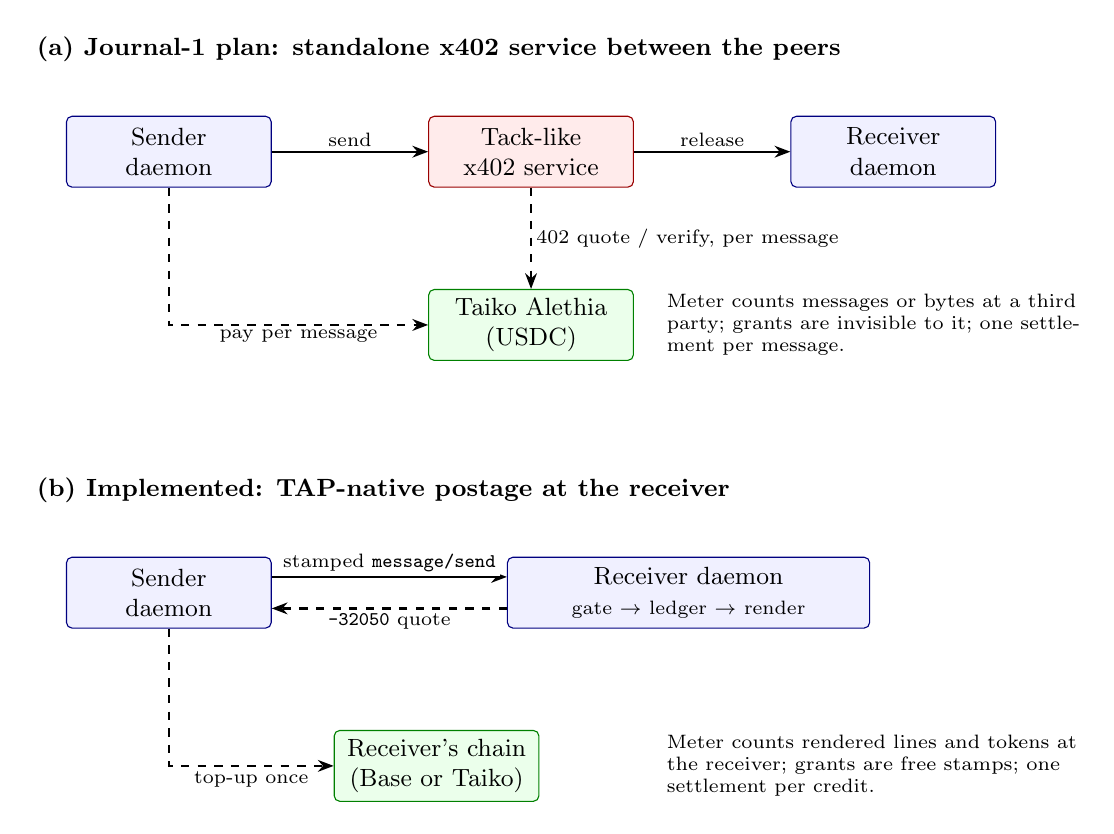
\begin{tikzpicture}[
  font=\small,
  box/.style={draw, rounded corners=2pt, minimum height=9mm, minimum width=26mm, align=center, inner sep=3pt},
  ext/.style={box, fill=red!8, draw=red!60!black},
  tap/.style={box, fill=blue!6, draw=blue!50!black},
  chain/.style={box, fill=green!8, draw=green!50!black},
  arr/.style={-{Stealth[length=2mm]}, thick},
  lbl/.style={font=\scriptsize, fill=white, inner sep=1.5pt},
]
% ---------------- (a) Journal-1 plan ----------------
\node[font=\bfseries\small, anchor=west] at (-6.4,1.9) {(a) Journal-1 plan: standalone x402 service between the peers};
\node[tap] (s1) at (-4.6,0.6) {Sender\\daemon};
\node[ext] (svc) at (0,0.6) {Tack-like\\x402 service};
\node[tap] (r1) at (4.6,0.6) {Receiver\\daemon};
\node[chain] (c1) at (0,-1.6) {Taiko Alethia\\(USDC)};
\draw[arr] (s1) -- node[lbl,above]{send} (svc);
\draw[arr] (svc) -- node[lbl,above]{release} (r1);
\draw[arr,dashed] (svc) -- node[lbl,right]{402 quote / verify, per message} (c1);
\draw[arr,dashed] (s1.south) |- node[lbl,below,pos=0.75]{pay per message} (c1.west);
\node[font=\scriptsize, align=left, anchor=west, text width=52mm] at (1.6,-1.6)
  {Meter counts messages or bytes at a third party; grants are invisible to it; one settlement per message.};
% ---------------- (b) Implemented ----------------
\begin{scope}[yshift=-5.6cm]
\node[font=\bfseries\small, anchor=west] at (-6.4,1.9) {(b) Implemented: TAP-native postage at the receiver};
\node[tap] (s2) at (-4.6,0.6) {Sender\\daemon};
\node[tap, minimum width=46mm] (r2) at (2.0,0.6) {Receiver daemon\\\scriptsize gate $\to$ ledger $\to$ render};
\node[chain] (c2) at (-1.2,-1.6) {Receiver's chain\\(Base or Taiko)};
\draw[arr] ([yshift=2mm]s2.east) -- node[lbl,above]{stamped \code{message/send}} ([yshift=2mm]r2.west);
\draw[arr,dashed] ([yshift=-2mm]r2.west) -- node[lbl,below]{\code{-32050} quote} ([yshift=-2mm]s2.east);
\draw[arr,dashed] (s2.south) |- node[lbl,below,pos=0.75]{top-up once} (c2.west);
\node[font=\scriptsize, align=left, anchor=west, text width=52mm] at (1.6,-1.6)
  {Meter counts rendered lines and tokens at the receiver; grants are free stamps; one settlement per credit.};
\end{scope}
\end{tikzpicture}
\caption{Placement of the attention meter. (a)~The first progress journal proposed a
standalone x402 service between the peers. (b)~The implemented design places metering,
pricing and postage inside the receiver's daemon, where attention is actually spent and
where identity and grants already live; the chain is touched once per credit, not once per
message.}
\label{fig:pivot}
\end{figure}

\subsection{Design principles}
\label{sec:design-principles}

The principles below were written down before the implementation began and were used to
settle the many smaller decisions that follow. Each is stated with the requirement it
serves.

\begin{enumerate}[label=P\arabic*.]
  \item \textbf{Meter where the cost lands.} Attention is accounted at the moment a line is
        rendered into a host context, from the same render plan the host uses, so the ledger
        can never disagree with what the agent saw (FR3, FR11).
  \item \textbf{Compress before you charge.} Coalescing and escalation-first rendering come
        first, because they eliminate most of the waste at no cost to anyone and because
        pricing without a unit of measurement is guesswork. Only after the ledger exists is
        it meaningful to publish a price (FR1--FR4).
  \item \textbf{Escalations outrank everything.} No mechanism---cap, coalescing, quota---may
        hide an escalation. Paid priority stamps and pending approvals are always rendered
        and never folded (FR2, FR9, FR10).
  \item \textbf{Never lose a message; fail open.} Metering may fold notifications into
        summaries; it may not drop messages. If a quota or ledger lookup fails, the batch
        passes through unmetered (NFR3).
  \item \textbf{Social trust precedes economic trust.} A grant is a free stamp. Postage
        exists for un-granted peers, and for granted peers who want more than the grant
        gives (a wake-up, or lines beyond the quota) (FR6, FR9, FR10).
  \item \textbf{Pay once, spend many.} One on-chain payment opens a credit; stamps are
        debited off-chain under a local mutex. Nothing in the per-message path touches the
        chain (FR7).
  \item \textbf{Opt in, and be machine-readable when you say no.} Enforcement is off by
        default; when it rejects, the rejection carries everything the sender needs to fix
        the situation without a human reading logs (FR5, NFR1).
  \item \textbf{Idempotent under crash and redelivery.} Every step that moves value or
        state is keyed so that a retry after a crash converges rather than double-charges
        (NFR2).
\end{enumerate}

\subsection{Pipeline overview}

Figure~\ref{fig:pipeline} shows where each mechanism sits in the inbound path. The gate
(\S\ref{sec:design-pricing}, \S\ref{sec:design-postage}) runs before anything is logged;
coalescing (\S\ref{sec:design-coalescing}) runs at enqueue; quota folding
(\S\ref{sec:design-priority}), accounting (\S\ref{sec:design-ledger}) and the
escalation-first render plan (\S\ref{sec:design-coalescing}) run at drain, inside the
daemon, so that every host receives the same batch.

\begin{figure}[htbp]
\centering
\resizebox{\textwidth}{!}{%
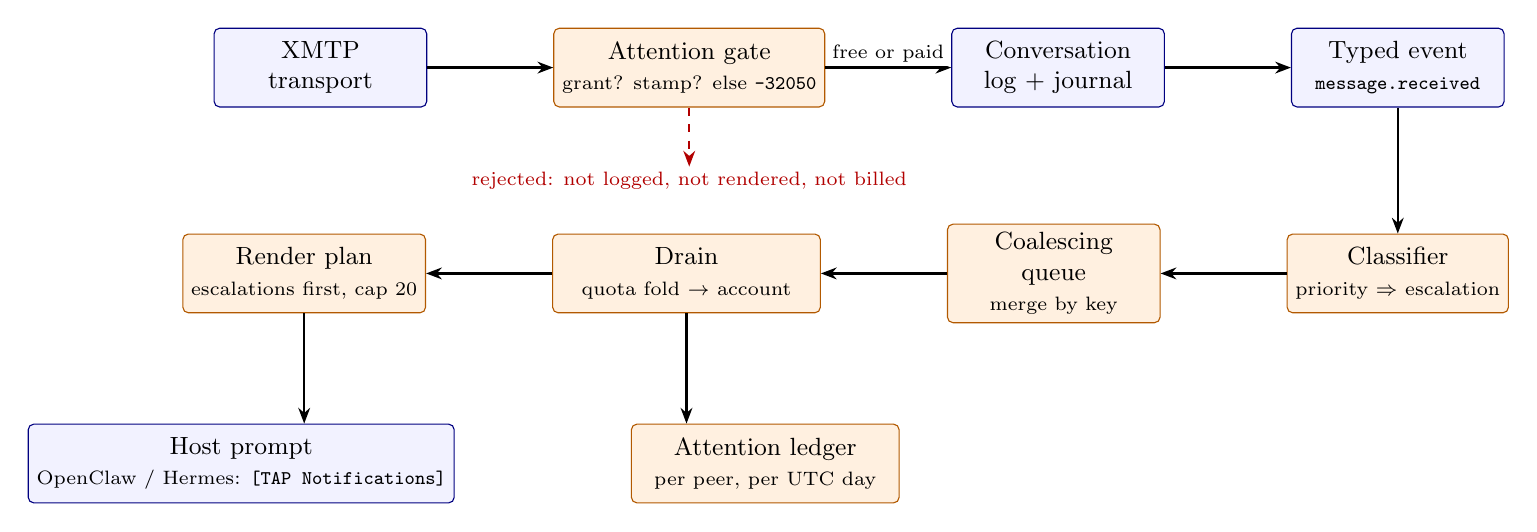
\begin{tikzpicture}[
  font=\small,
  node distance=7mm and 16mm,
  stage/.style={draw, rounded corners=2pt, minimum height=10mm, minimum width=27mm, align=center, inner sep=3pt, fill=blue!5, draw=blue!50!black},
  new/.style={stage, fill=orange!12, draw=orange!70!black},
  arr/.style={-{Stealth[length=2mm]}, thick},
  lbl/.style={font=\scriptsize, fill=white, inner sep=1.5pt},
]
\node[stage] (xmtp) {XMTP\\transport};
\node[new, right=of xmtp, minimum width=34mm] (gate) {Attention gate\\\scriptsize grant? stamp? else \code{-32050}};
\node[stage, right=of gate] (log) {Conversation\\log + journal};
\node[stage, right=of log] (evt) {Typed event\\\scriptsize \code{message.received}};
\node[new, below=16mm of evt] (cls) {Classifier\\\scriptsize priority $\Rightarrow$ escalation};
\node[new, left=of cls] (q) {Coalescing\\queue\\\scriptsize merge by key};
\node[new, left=of q, minimum width=34mm] (drain) {Drain\\\scriptsize quota fold $\to$ account};
\node[new, left=of drain] (plan) {Render plan\\\scriptsize escalations first, cap 20};
\node[stage, below=14mm of plan, xshift=-8mm, minimum width=48mm] (host) {Host prompt\\\scriptsize OpenClaw / Hermes: \code{[TAP Notifications]}};
\node[new, below=14mm of drain, xshift=10mm, minimum width=34mm] (ledger) {Attention ledger\\\scriptsize per peer, per UTC day};
\draw[arr] (xmtp) -- (gate);
\draw[arr] (gate) -- node[lbl,above]{free or paid} (log);
\draw[arr] (log) -- (evt);
\draw[arr] (evt) -- (cls);
\draw[arr] (cls) -- (q);
\draw[arr] (q) -- (drain);
\draw[arr] (drain) -- (plan);
\draw[arr] (plan.south) -- (host.north -| plan.south);
\draw[arr] (drain.south) -- (ledger.north -| drain.south);
\draw[arr, dashed, red!70!black] (gate.south) -- ++(0,-0.75) node[lbl, below, text=red!70!black]{rejected: not logged, not rendered, not billed};
\end{tikzpicture}%
}
\caption{Inbound path in the receiving daemon. Orange stages were added by this project.
A rejected message never reaches the log, the queue or the ledger. Everything from the
queue to the render plan runs inside \code{tapd}, so the CLI, OpenClaw and Hermes render
one canonical batch.}
\label{fig:pipeline}
\end{figure}

\subsection{Notification coalescing and escalation-first rendering}
\label{sec:design-coalescing}

\paragraph{Problem restated.}
The legacy queue appended one notification per event and the renderer emitted the first
twenty in arrival order. Fifty chat messages from three peers followed by one transfer
request produced twenty interleaved chat lines and a footer ``31 more TAP notifications
omitted''---with the approval request inside the 31.

\paragraph{Coalescing at enqueue.}
Each notification may carry a \code{coalesceKey} and a \code{coalesceStrategy}. When a
new notification arrives whose key is already buffered, it is merged \emph{in place}: the
entry keeps its buffer slot and identifier, its content becomes the newest event's
content, and, under the default \code{count} strategy, a \code{count} accumulates. The
alternative \code{replace} strategy swaps content without counting; it is used for state
transitions such as an action going from pending to completed, which is one thing changing
rather than many things repeating. Chat from one connection is keyed
\code{msg:<connectionId>}, so a flood from Alice becomes a single line
``\code{New message from Alice: \ldots (x334)}''. The design choice to keep the
\emph{first-arrival} slot but the \emph{newest} content is deliberate: the slot preserves
fairness of ordering across peers, while the content shows the operator the most recent
state of the conversation.

Coalescing happens at enqueue rather than at drain for two reasons. First, the queue is
bounded (1{,}000 entries, oldest dropped) as a safety measure against a host that never
drains; merging at enqueue means a flood from one peer occupies one slot and cannot evict
other peers' notifications. Second, a per-key index kept in step with the buffer makes
the merge $O(1)$; the index is cleared on drain and pruned on eviction so that a stale
mapping can never merge new events into an entry that is no longer buffered.

\paragraph{Escalation-first render plan.}
Rendering was refactored into a pure function that returns a \emph{plan}
(\code{planNotificationRender}): the lines that will be rendered, the entries omitted
past the cap, and a footer. The plan drops empty one-liners, then stable-partitions escalations ahead of all
other types (preserving arrival order within each class), caps at twenty, and summarises
the omitted tail \emph{grouped by peer and type with event counts}
(``\code{omitted: 334 messages from Alice, 2 auto-replies}'') rather than as an opaque
number. Because the plan is a value rather than a side effect, the OpenClaw host renders
exactly it, the Hermes Python plugin mirrors it, and the accounting step
(\S\ref{sec:design-ledger}) bills from it. This single-source-of-truth property is what
satisfies FR11.

\paragraph{Priority messages are never coalesced.}
A message whose stamp paid the priority tier (\S\ref{sec:design-priority}) is classified
as an escalation with a 400-character excerpt instead of 80 and carries no coalesce key.
A paid wake-up must remain individually visible; collapsing two of them into one line
would silently refund nothing and hide one.

\subsection{The attention ledger}
\label{sec:design-ledger}

The ledger answers one question: \emph{what has each peer cost me?} It is a file
(\path{<dataDir>/attention-ledger.json}) of UTC-day buckets, each holding per-peer
statistics and a total. The unit of account is defined by the render plan: for every
rendered line the ledger adds one to \code{notificationsRendered} and
$\lceil \text{chars}/4 \rceil$ to \code{tokensInjected}; escalations increment
\code{escalations}; omitted entries add their event counts to
\code{overflowSuppressed}. Peers are keyed \code{<chain>\#<agentId>}, the same key the
postage ledger uses so the two can be joined; block overhead and events with no peer (a
pending-action escalation, for instance) are booked to an \code{unattributed} row.

Three properties are intentional. The ledger records \emph{rendered} lines, not received
messages, so a peer whose flood coalesced into one line is billed one line---the ledger
measures attention actually spent, which is what P1 demands and what makes quota
enforcement (\S\ref{sec:design-priority}) fair. Retention is thirty days with pruning on
write, so the file is bounded. And the ledger is written only by the transport-owning
daemon, under a process-local mutex and the repository's atomic \code{tmp + rename}
pattern, so it inherits the single-writer discipline TAP already imposes on the trust
store. \code{tap attention show} is a pure local read and starts no transport, in keeping
with the ``fat CLI'' rule.

\subsection{Attention pricing and the \code{-32050} quote}
\label{sec:design-pricing}

\paragraph{Publishing prices.}
An agent's price list lives in \code{config.yaml} under \code{attention.pricing} and is
copied into the registration file as \code{trustedAgentProtocol.attention} on the next
\code{tap register update}, with a \code{version}, a \code{currency} (USDC), an optional
CAIP-2 \code{chain}~\cite{caip2} and a map of tiers to decimal amounts. Three tiers are defined:
\code{grantHolder} (documentary---grant holders are free by construction),
\code{standard} (the price a stamp must cover to buy delivery) and \code{priority} (the
price that additionally buys a wake-up). Putting prices in the registration file rather
than inventing a new discovery message reuses the existing, cached
(\raisebox{0.3ex}{\textasciitilde}24\,h) resolution path: a sender learns a peer's prices
with \code{tap identity resolve}, and \code{tap message send --dry-run} previews the cost
and whether a stamp would be attached.

\paragraph{The gate.}
With \code{attention.enforce: true}, an inbound \code{message/send} passes through a gate
before the conversation log. If the sender holds an active \code{message/send} grant,
the message is free (FR6). Otherwise the gate looks for a stamp
(\S\ref{sec:design-postage}); if none is present, or the stamp does not cover the
\code{standard} price, the message is rejected with
\code{AttentionPaymentRequiredError}, which the transport maps to JSON-RPC
\code{-32050} with \code{error.data.attention} holding the quote and
\code{error.data.postage} holding a reason from the closed set
\{\code{missing\_stamp}, \code{unpriced}, \code{unknown\_credit},
\code{seq\_replayed}, \code{below\_price}, \code{insufficient\_credit}\}. The reason set
was chosen so that a sender can decide mechanically whether a top-up would help
(\code{insufficient\_credit}, \code{unknown\_credit}) or whether the stamp itself is wrong.

Two details carry the compatibility requirement. First, if enforcement is on but no
\code{standard} price is published, the gate degrades to ``granted peers only'' rather
than accepting any stamp: an unpriced receiver cannot be bought. Second, the rejection
marks the request journal entry \emph{completed} before throwing, so a later full-history
sync replays the duplicate short-circuit instead of re-running enforcement per replay.

\subsection{Prepaid postage}
\label{sec:design-postage}

Postage is the two-step model from the research note~\cite{tap-research-note}
instantiated between two peers with no facilitator. Figure~\ref{fig:postage} shows the
lifecycle.

\begin{figure}[htbp]
\centering
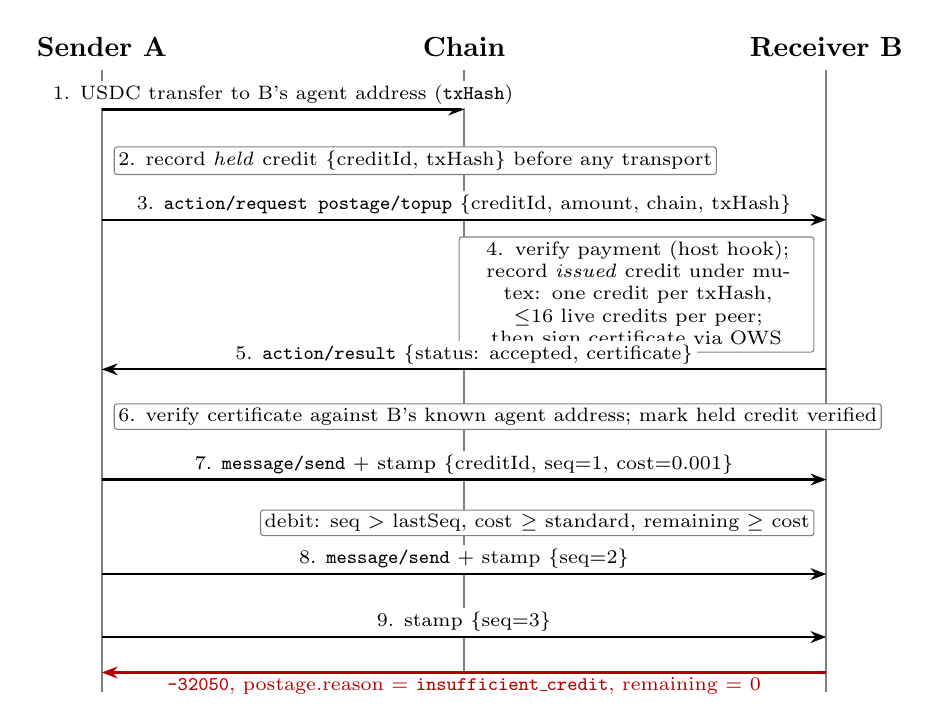
\begin{tikzpicture}[
  font=\small,
  arr/.style={-{Stealth[length=2mm]}, thick},
  lbl/.style={font=\scriptsize, fill=white, inner sep=1.5pt, align=center},
]
\def\L{0}\def\C{4.6}\def\R{9.2}
\node[font=\bfseries] (sT) at (\L,0) {Sender A};
\node[font=\bfseries] (cT) at (\C,0) {Chain};
\node[font=\bfseries] (rT) at (\R,0) {Receiver B};
\draw[thick, gray] (\L,-0.3) -- (\L,-8.2);
\draw[thick, gray] (\C,-0.3) -- (\C,-8.2);
\draw[thick, gray] (\R,-0.3) -- (\R,-8.2);
% 1 pay
\draw[arr] (\L,-0.8) -- node[lbl,above]{1. USDC transfer to B's agent address (\code{txHash})} (\C,-0.8);
% 2 record held
\node[lbl, anchor=west, draw=gray, rounded corners=1pt] at (\L+0.15,-1.45) {2. record \emph{held} credit \{creditId, txHash\} before any transport};
% 3 topup request
\draw[arr] (\L,-2.2) -- node[lbl,above]{3. \code{action/request postage/topup} \{creditId, amount, chain, txHash\}} (\R,-2.2);
% 4 verify + record issued + sign
\node[lbl, anchor=east, draw=gray, rounded corners=1pt, text width=44mm] at (\R-0.15,-3.15)
  {4. verify payment (host hook); record \emph{issued} credit under mutex: one credit per txHash, $\le$16 live credits per peer; then sign certificate via OWS};
% 5 result
\draw[arr] (\R,-4.1) -- node[lbl,above]{5. \code{action/result} \{status: accepted, certificate\}} (\L,-4.1);
\node[lbl, anchor=west, draw=gray, rounded corners=1pt] at (\L+0.15,-4.7) {6. verify certificate against B's known agent address; mark held credit verified};
% 7 stamped sends
\draw[arr] (\L,-5.5) -- node[lbl,above]{7. \code{message/send} + stamp \{creditId, seq=1, cost=0.001\}} (\R,-5.5);
\node[lbl, anchor=east, draw=gray, rounded corners=1pt] at (\R-0.15,-6.05) {debit: seq $>$ lastSeq, cost $\ge$ standard, remaining $\ge$ cost};
\draw[arr] (\L,-6.7) -- node[lbl,above]{8. \code{message/send} + stamp \{seq=2\}} (\R,-6.7);
\draw[arr] (\L,-7.5) -- node[lbl,above]{9. stamp \{seq=3\}} (\R,-7.5);
\draw[arr, red!70!black] (\R,-7.95) -- node[lbl,below]{\code{-32050}, postage.reason = \code{insufficient\_credit}, remaining = 0} (\L,-7.95);
\end{tikzpicture}
\caption{Postage lifecycle between two connected agents. One on-chain payment (1) opens a
credit; all later steps are off-chain. Steps 7--9 correspond to the teammate's Experiment~2
(Section~\ref{sec:eval-postage}).}
\label{fig:postage}
\end{figure}

\paragraph{Top-up as a TAP action.}
A top-up is an ordinary \code{action/request} of type \code{postage/topup}, handled by a
TAP app. This was the natural fit: the app registry, the request journal, the
result-waiter machinery and the conversation log all apply without special cases, and the
same handlers ship both as a built-in of \code{core} and as the standalone package
\code{@trustedagents/app-postage} for hosts that assemble their own app set. The handler
receives its capabilities through a narrow, host-injected extension
(\code{ctx.extensions.postage}: \code{recordIssued}, \code{issuedFor},
\code{signCredit}, \code{verifyTopup}) rather than through the generic app storage,
precisely so that top-ups and stamp debits are serialised by \emph{one} ledger mutex.

\paragraph{Pay first, then ask.}
The sender pays before it sends the top-up request, and records the \emph{held} credit
locally before any transport action. The ordering is chosen for recoverability: the
payment is irreversible, so whatever fails afterwards, the sender's ledger holds the
\code{creditId}/\code{txHash} pair needed to retry, and the receiver's handler is
idempotent per \code{creditId}---a retry after a timeout returns the original
certificate and never opens a second credit. A definitive rejection by the peer removes
the held record so that it cannot feed auto-stamping.

\paragraph{The credit certificate.}
On acceptance the receiver signs, through its OWS signing provider, an EIP-191 personal
signature~\cite{eip191} over the keccak digest of the ABI-encoded facts
\code{(creditId, issuerChain, issuerAgentId, holderAgentId, amountMicros, txHash)}. The
holder verifies it against the issuer's agent address already recorded in its contact
entry---the same scheme and the same trust anchor that invites use. The certificate is the
holder's portable proof that the credit exists and is bound to a specific payment; it is
not needed on the per-message path.

\paragraph{Stamps and the debit rule.}
Once a verified held credit exists, \code{sendMessage} attaches a stamp
\code{\{creditId, seq, cost\}} to the \code{trustedAgent} metadata of every
\code{message/send} to that peer automatically, drawing on the oldest credit whose
remaining balance covers the cost, and persists the incremented \code{seq} and spend
\emph{before} the stamp is returned---so a crash wastes one sequence value rather than
reusing one. On the receiving side a debit succeeds only if the credit exists and belongs
to this peer, \code{cost} is well-formed and at least the \code{standard} price,
\code{seq} is strictly greater than the credit's \code{lastSeq}, and the remaining balance
covers \code{cost}. The whole check-and-spend runs under the ledger mutex. The strictly
increasing sequence is the replay defence: a captured stamp cannot be presented twice,
and there is no nonce set to store or expire. The one exception is deliberate: a stamp
with \code{seq == lastSeq} \emph{and} the same delivery key as the last debit is accepted
without charge, because it is the crash-window redelivery of the message that already
paid.

\paragraph{Why stamps live in \code{message/send} metadata.}
Carrying the stamp inside the existing message rather than as a separate action keeps the
per-message path to one wire message, and lets a pre-project receiver ignore it: metadata
it does not understand is simply not read (NFR1).

\subsection{Priority stamps and notification quotas}
\label{sec:design-priority}

The final mechanism separates the two prices identified in
Section~\ref{sec:background}---context and wake-ups---and gives grant holders a metered
free tier.

\paragraph{Priority buys the wake-up, the grant buys delivery.}
A stamp whose \code{cost} meets the receiver's published \code{priority} price is booked
at tier \code{priority}. The classifier then emits an \emph{escalation} with a
400-character excerpt, the queue never coalesces it, the render plan places it first,
and OpenClaw's escalation watcher calls \code{requestHeartbeatNow()} so the agent wakes
immediately (Hermes shows it on the next turn). Critically, this applies to grant holders
too: the gate exempts a grant holder from paying for delivery, but a priority-value stamp
from a grant holder is still debited and still buys the wake-up
(\code{chargeOptionalPriorityStamp}). The grant encodes ``I will read what you send'';
the priority stamp encodes ``interrupt me now''---these are different permissions and are
priced separately. Any failure in the optional priority path degrades silently to plain
grant delivery: a grant holder is never rejected over a malformed stamp.

\paragraph{The weekly quota.}
A \code{message/send} grant may carry the constraint \code{notificationsPerWeek: N}. At
drain time, before accounting and before any host renders, the daemon groups the batch's
\code{info} notifications by peer, asks the attention ledger how many lines that peer had
rendered in the trailing seven UTC days, and---if the peer is at or over quota---replaces
the peer's info notifications with one \code{summary} line
(``\code{12 notifications from Alice folded --- weekly notification quota reached
(20/week)}'') whose \code{count} preserves the number of underlying events. The messages
are still delivered and still in the conversation log; only their per-line claim on
attention is withdrawn. Escalations are excluded from folding by construction (P3). When
several active grants disagree, the most permissive wins, because all of them were issued
by this same agent. If the trust store or ledger cannot answer, the batch passes through
unfolded (P4).

Quota enforcement is placed in the drain rather than in the renderer for the same reason
accounting is: it must happen once, in the daemon, so that OpenClaw, Hermes and the
ledger all see the same folded batch. It counts \emph{rendered} lines rather than
received messages so that a peer whose chatter already coalesced is not penalised twice.
Together the two mechanisms make the grant's free tier finite and let the peer buy past it
with postage---which is exactly the relationship P5 asks for.

\section{Implementation}
\label{sec:implementation}

All implementation work described in this section is the author's. It lives on the branch
\path{feat/phase1-notification-coalescing} of the project repository and is submitted as
pull request~\#1~\cite{tap-pr1}. Relative to the branch point (\code{e52bb66}, the
upstream \code{0.2.0-beta.7} release), the implementation commits touch 91~files with
approximately 8{,}200 lines added and 140 removed, of which roughly 3{,}200 lines are
production source, 4{,}300 lines are tests, and the remainder is documentation.

\subsection{Increments}

The work was landed as five increments, each of which left the repository lint-clean,
type-clean and green under \code{bun run test}, in the dependency order that principle~P2
prescribes. Table~\ref{tab:increments} summarises them; the full commit list is in
Appendix~\ref{app:commits}.

\begin{table}[htbp]
\centering\small
\caption{Implementation increments, in landing order.}
\label{tab:increments}
\begin{tabularx}{\textwidth}{@{}l>{\raggedright\arraybackslash}X>{\raggedright\arraybackslash}X@{}}
\toprule
\textbf{Increment} & \textbf{Scope} & \textbf{Principal modules} \\
\midrule
1. Coalescing &
Coalesce at enqueue; escalation-first render plan with grouped overflow summary; flood demo script; skill documentation of the new block semantics. &
\path{tapd/notification-queue.ts}, \path{tapd/notification-format.ts}, \path{scripts/demo-notification-flood.ts} \\
2. Ledger &
File-backed per-peer attention ledger; accounting on drain derived from the canonical render plan; \code{tap attention show}. &
\path{core/attention/ledger.ts}, \code{tapd/daemon.ts}, \path{cli/commands/attention-show.ts} \\
3. Pricing &
\code{attention} block in config and registration file (validated on both sides); price discovery in \code{identity resolve}; \code{--dry-run} cost preview; \code{-32050} rejection of un-granted \code{message/send}. &
\code{core/config/*}, \path{core/identity/registration-file.ts}, \path{core/common/errors.ts}, \path{core/runtime/service.ts}, \path{core/transport/xmtp.ts} \\
4. Postage &
Credit ledger (issued/held), stamps, credit certificates; \code{postage/topup} and \code{postage/balance} handlers; auto-stamping in \code{sendMessage}; top-up orchestration; \code{tap postage topup/balance}; \code{@trustedagents/app-postage}; \code{tapd} routes. &
\code{core/postage/*}, \code{app-postage/}, \path{cli/commands/postage-*.ts}, \path{tapd/http/routes/postage.ts} \\
5. Priority \& quota &
Priority tier on stamps; escalation classification with 400-char excerpt; wake-up in OpenClaw; \code{notificationsPerWeek} folding at drain; \code{--priority} threaded through CLI, \code{tapd}, OpenClaw tool and Hermes plugin. &
\path{tapd/notification-quota.ts}, \path{tapd/notification-classifier.ts}, \path{openclaw-plugin/escalation-watcher.ts}, \path{cli/assets/hermes/plugin/} \\
\bottomrule
\end{tabularx}
\end{table}

\subsection{Data structures}

\paragraph{Notifications.}
\code{TapNotification} gained three fields (\code{coalesceKey}, \code{coalesceStrategy}
and \code{count}), all optional so that a batch produced by an older daemon renders
unchanged. The queue keeps a \code{Map<coalesceKey, entry>} beside
the array buffer; the invariant that the map never points at an entry outside the buffer
is maintained at exactly two places (drain and max-size eviction) and is covered by unit
tests.

\paragraph{Attention ledger file.}
Listing~\ref{lst:ledger} shows the on-disk shape. Day buckets are keyed by UTC date so
that the weekly window (\code{renderedInWindow(peer, 7)}) is a simple prefix comparison
over keys, and pruning on write bounds the file at the retention period.

\begin{lstlisting}[language=json,caption={Shape of \code{attention-ledger.json} (abridged).},label={lst:ledger}]
{
  "version": 1,
  "identity": { "chain": "eip155:8453", "agentId": 1 },
  "days": {
    "2026-08-27": {
      "peers": {
        "eip155:8453#11": { "notificationsRendered": 1, "tokensInjected": 24,
                            "escalations": 0, "overflowSuppressed": 0 },
        "unattributed":   { "notificationsRendered": 1, "tokensInjected": 31,
                            "escalations": 1, "overflowSuppressed": 0 }
      },
      "totals": { "notificationsRendered": 2, "tokensInjected": 55,
                  "escalations": 1, "overflowSuppressed": 0 }
    }
  }
}
\end{lstlisting}

\paragraph{Postage state.}
\path{<dataDir>/apps/postage/state.json} holds two maps keyed by \code{creditId}:
\code{issued} (credits peers bought \emph{with} this agent; fields \code{peer},
\code{amount}, \code{spent}, \code{lastSeq}, \code{lastStampKey}, \code{txHash},
\code{certificate}) and \code{held} (credits this agent bought \emph{at} peers; fields
\code{nextSeq}, \code{certificateVerified} in place of \code{lastSeq}). Amounts are
decimal strings with at most six places and are converted to integer micro-units
(\code{bigint}) for every arithmetic operation; no floating point touches money.

\subsection{Wire formats}

\paragraph{Registration file.}
The \code{trustedAgentProtocol.attention} block (Listing~\ref{lst:regfile}) is validated
by the same \code{validateRegistrationFile} that already checks the XMTP endpoint, on both
the publishing and the resolving side, so a malformed price list is rejected before it
can be cached.

\begin{lstlisting}[language=json,caption={Attention block in the ERC-8004 registration file.},label={lst:regfile}]
"trustedAgentProtocol": {
  "agentAddress": "0x...",
  "attention": {
    "version": "1.0",
    "currency": "USDC",
    "chain": "eip155:167000",
    "pricing": { "grantHolder": "0", "standard": "0.001", "priority": "0.01" }
  }
}
\end{lstlisting}

\paragraph{Rejection.}
The transport previously collapsed any service error into the generic JSON-RPC
\code{-32603}. It now preserves \code{AttentionPaymentRequiredError} as \code{-32050}
with structured \code{data} (Listing~\ref{lst:reject}), and the sending side raises a
\code{TransportRpcError} that keeps \code{rpcCode} and \code{rpcData} so that callers
can react programmatically. The CLI and \code{tapd} translate the same object to HTTP
\code{402 attention\_payment\_required}.

\begin{lstlisting}[language=json,caption={A \code{-32050} rejection as seen by the sender.},label={lst:reject}]
{
  "jsonrpc": "2.0", "id": "req-...",
  "error": {
    "code": -32050,
    "message": "attention payment required: ...",
    "data": {
      "attention": { "version": "1.0", "currency": "USDC",
                     "chain": "eip155:167000",
                     "pricing": { "standard": "0.001", "priority": "0.01" } },
      "postage": { "reason": "insufficient_credit", "creditId": "...",
                   "remaining": "0", "required": "0.001" }
    }
  }
}
\end{lstlisting}

\paragraph{Stamp.}
A stamp is a \code{postage} object with three fields, \code{creditId}, \code{seq} and
\code{cost}, inside the existing \code{trustedAgent} metadata of a \code{message/send}
(for example \code{\{"creditId": "c-7f3a", "seq": 3, "cost": "0.001"\}}).
\path{extractPostageStamp} guards only shape; economic validity is the ledger's decision,
so a malformed stamp can never crash enforcement.

\subsection{The service gate}

The gate is a single block in \code{TapMessagingService.processInboundRequest}, placed
after contact resolution and duplicate detection but before the conversation log. Its
ordering constraints are the subtle part of the implementation and are worth stating:

\begin{enumerate}
  \item Enforcement runs only for \code{message/send} and only when
        \code{config.attention.enforce} is true.
  \item A rejected request marks its journal entry \code{completed} \emph{before} throwing,
        so that a full-history sync hits the duplicate short-circuit rather than re-running
        enforcement per replay.
  \item An accepted stamp completes the journal entry \emph{after} the conversation log.
        A crash between the debit and that completion redelivers the message with its
        journal entry pending; the ledger's \code{lastStampKey} lets that exact redelivery
        pass idempotently, and the event is emitted even though the delivery is a duplicate,
        because otherwise the receiver would keep the money and drop what it bought.
  \item For a grant holder the gate does not reject; it calls
        \code{chargeOptionalPriorityStamp}, which debits only if the stamp meets the
        \code{priority} price and swallows every failure.
\end{enumerate}

The \code{message.received} event carries an optional \code{postage: \{tier, cost\}}
reference only when a stamp was actually debited, so downstream consumers cannot
mistake a free delivery for a paid one.

\subsection{Top-up orchestration}

\code{topUpPostage} runs under the service's execution mutex and inside a transport
session. It (i)~validates the amount; (ii)~pays through the host's
\code{executeTransfer} hook---the same hook \code{tap transfer} uses, so the payment is an
ordinary USDC transfer on the contact's chain, signed through OWS; (iii)~records the held
credit; (iv)~sends the \code{postage/topup} action and waits for the result with a waiter
that settles on \emph{any} result for the request, not only one carrying the
\code{actionId}, so that a pre-postage peer's \code{UNSUPPORTED\_ACTION} reply is read as
a definitive rejection rather than a timeout; (v)~verifies the returned certificate
against the contact's agent address and marks the held credit verified. A transport
failure after payment is returned as \code{status: pending} with the \code{txHash}
rather than thrown, because the payment has happened and the caller must be told so.

\subsection{Host surfaces}

Following the ``thin plugin, fat CLI'' rule, only operations that need the live transport
were added to the plugin surface. Table~\ref{tab:surfaces} lists the new commands.

\begin{table}[htbp]
\centering\small
\caption{Operator-facing surfaces added by the project.}
\label{tab:surfaces}
\begin{tabularx}{\textwidth}{@{}l>{\raggedright\arraybackslash}Xl@{}}
\toprule
\textbf{Surface} & \textbf{Behaviour} & \textbf{Transport?} \\
\midrule
\code{tap attention show} & Per-peer attention usage over the retained window, highest token spend first; reads \code{attention-ledger.json}. & No \\
\code{tap identity resolve <id>} & Now prints the peer's advertised \code{attention} block. & No \\
\code{tap register update} & Publishes \code{attention.pricing} from config into the registration file. & No (on-chain) \\
\code{tap message send --dry-run} & Shows the peer's price, \code{postage\_remaining} and \code{would\_stamp}; sends nothing. & No \\
\code{tap message send --priority} & Pays the peer's \code{priority} price so the message escalates and may wake the peer. & Yes \\
\code{tap postage topup <peer> --amount} & Pays USDC on-chain, opens a credit, stores the certificate; \code{--yes}, \code{--dry-run}. & Yes \\
\code{tap postage balance [--peer]} & Credits held at peers and issued to peers. & No \\
\code{tap\_gateway send\_message \{priority\}} & OpenClaw and Hermes tool flag mirroring \code{--priority}. & Yes \\
\code{tapd} \code{POST /api/postage/*}, \code{/api/notifications/drain} & Daemon routes behind which the CLI and plugins operate. & --- \\
\bottomrule
\end{tabularx}
\end{table}

The Hermes Python plugin, which mirrors the render plan rather than importing it, was
extended to render the \code{(xN)} suffix and to forward the \code{priority} flag, and its
Python tests (\code{test\_client.py}) pin both behaviours; the folded-quota summary needs no
host-side change because it arrives as an ordinary \code{summary} notification.

\subsection{Testing}

Testing follows the repository's existing three tiers.

\paragraph{Unit.} New suites cover the queue invariants (merge in place, index pruned on
eviction, \code{replace} strategy never counts), the render plan (partition stability,
grouped summary text, cap), the attention ledger (bucketing, retention, window counts),
the postage ledger (idempotent \code{recordIssued}, one credit per \code{txHash}, per-peer
cap, replay rejection, redelivery exception, no double spend under concurrent debits), the
certificate (sign/verify round trip; wrong signer rejected), the payload parsers, the
quota fold (escalations excluded; fail-open on lookup error), and the OpenClaw escalation
watcher.

\paragraph{Service.} \code{service.test.ts} exercises the gate against a mocked transport:
enforcement off is a no-op; un-granted and unstamped is rejected with a quote; a grant
exempts; a valid stamp debits; an exhausted credit yields \code{insufficient\_credit}; a
grant holder's priority stamp buys the escalation tier.

\paragraph{Mock end-to-end.} Three new phases were added to the canonical scenario list
shared by both E2E suites (Table~\ref{tab:e2e}). They run over the loopback transport on
every pull request. They are deliberately \emph{not} mirrored into the live-mainnet suite
yet: the key assertions are negative (``B never logged the message''), which are
timing-flaky over real XMTP, and both mechanisms are opt-in so live behaviour is
unchanged. This gap is recorded as a follow-up in the pull request.

\begin{table}[htbp]
\centering\small
\caption{Mock E2E scenarios added (phases 6--8 of \code{packages/cli/test/e2e/scenarios.ts}).}
\label{tab:e2e}
\begin{tabularx}{\textwidth}{@{}l>{\raggedright\arraybackslash}X@{}}
\toprule
\textbf{Phase} & \textbf{Scenarios} \\
\midrule
6 Attention &
Preview cost with \code{--dry-run}; enable enforcement on B; send without grant rejected with quote; \code{message/send} grant exempts sender. \\
7 Postage &
Revoke grant so postage applies; top-up buys credit with signed certificate; auto-stamped message delivers and debits; exhausted credit rejected with top-up quote; \code{postage balance} shows held and issued credits on both sides. \\
8 Wake \& quota &
Publish a \code{priority} price; priority stamp escalates with a 400-char excerpt; over-quota grant holder's chatter folds to one summary line; grant holder's priority stamp still buys the wake-up. \\
\bottomrule
\end{tabularx}
\end{table}

\subsection{Documentation}

Every new command and flag was added to the canonical skill file
\path{skills/trusted-agents/SKILL.md}, which the OpenClaw plugin and the Hermes installer
copy at build time, and the \code{notificationsPerWeek} constraint to
\path{references/permissions-v1.md}. The skill's ``how to read the block'' guidance was
rewritten so that an agent encountering \code{(xN)}, a folded-quota summary or a
``Priority message from'' escalation knows what each means and how to act. The
repository's \code{README} and \code{Agents.md} were aligned in a final documentation
commit.

\section{Evaluation}
\label{sec:evaluation}

\subsection{Attribution and method}

The evaluation was designed and executed by the project teammate, Zhang Hanyu, and is
recorded in \path{evaluation/results.md} together with the benchmark scripts
\path{scripts/benchmark-attention.ts} and \path{scripts/benchmark-postage.ts}, merged
into the implementation branch as pull request~\#2 (merge commit
\code{0330091})~\cite{tap-eval}. This section reproduces his results without alteration
and adds the author's interpretation in the light of the design. Where the two are mixed
the text says so.

The evaluation asks three questions, one per requirement group:

\begin{enumerate}[label=Q\arabic*.]
  \item Does coalescing with escalation-first rendering reduce the notification context
        injected into the receiver's prompt, and keep the escalation visible? (FR1, FR2)
  \item Does prepaid postage impose an economic limit on repeated delivery? (FR5, FR7)
  \item Do priority messages remain visible when ordinary notifications are limited by a
        quota? (FR9, FR10)
\end{enumerate}

The experiments were run on Windows against the branch as merged. The teammate reports
that the project built after minor local compatibility fixes to TypeScript typing and
build scripts, but that the OWS native package
\path{@silicon-intern/ows-core-win32-x64-msvc} was unavailable in that environment. This
constrained which mechanisms could be exercised end to end and is discussed under Q3 and
in Section~\ref{sec:limitations}.

\subsection{Experiment 1: notification flood and attention reduction}
\label{sec:eval-flood}

\paragraph{Set-up.}
Three peer agents send $N$ ordinary chat messages in round-robin, after which one
transfer request requiring approval arrives. The arrival order is the worst case for a
FIFO renderer: the escalation is last. Two pipelines are compared on identical event
streams: the \emph{legacy} pipeline (append-only queue, per-event rendering, hard cap of
twenty lines, opaque ``$N$ more omitted'' footer) and the \emph{new} pipeline (coalescing
queue, escalation-first plan, grouped summary). $N \in \{10, 50, 100, 500, 1000\}$.
Token cost is estimated with the project's existing approximation
$\lceil \text{characters}/4 \rceil$; the figures are therefore estimated tokens, not
tokenizer counts. ``Escalation visible'' records whether the transfer request appears as a
rendered line.

\paragraph{Results.}

\begin{table}[htbp]
\centering\small
\caption{Experiment 1: estimated tokens injected per prompt and escalation visibility
(teammate's results, reproduced verbatim).}
\label{tab:flood}
\begin{tabular}{@{}rrrrll@{}}
\toprule
\textbf{Messages} & \textbf{Legacy tokens} & \textbf{New tokens} & \textbf{Reduction} & \textbf{Legacy escal.} & \textbf{New escal.} \\
\midrule
10   & 256 &  97 & 62.1\% & Visible & Visible \\
50   & 482 &  98 & 79.7\% & Hidden  & Visible \\
100  & 482 &  98 & 79.7\% & Hidden  & Visible \\
500  & 482 & 100 & 79.3\% & Hidden  & Visible \\
1000 & 483 & 100 & 79.3\% & Hidden  & Visible \\
\bottomrule
\end{tabular}
\end{table}

\paragraph{Interpretation.}
Three observations follow directly from the numbers, and each traces to a specific design
decision.

First, the new pipeline's cost is essentially \emph{flat}: 97--100 estimated tokens from
10 to 1000 messages. This is the coalescing invariant of \S\ref{sec:design-coalescing} at
work---three peers produce three counted lines regardless of $N$, and the only growth is
the width of the \code{(xN)} suffix as the count gains digits. The legacy pipeline
saturates at 482--483 tokens from $N=50$ onward because its cap of twenty lines is
already full at 50 messages; the reduction therefore stabilises at about 79\% rather than
growing without bound, which is the honest way to read the table. At $N=10$ the legacy
renderer is under its cap, so the gap is smaller (62.1\%).

Second, the legacy pipeline \emph{hides the escalation} at every flood size of 50 and
above, exactly the failure that motivated FR2: twenty chat lines fill the cap and the
approval request falls into the footer. The new pipeline renders it in every case,
because the plan partitions escalations first. The evaluation thus confirms both halves
of the coalescing increment---less context, and the right context.

Third, the absolute numbers matter less than their shape. A saving of roughly 380
estimated tokens per prompt is modest in isolation; but the block is injected on
\emph{every} prompt while the notifications are pending, in a streaming host it is
injected on every wake, and without coalescing the block's size is set by the most
talkative peer rather than by the operator. Bounding it is what makes a per-peer
attention price meaningful at all (principle P2).

\paragraph{Reproducibility.}
The scenario is synthetic and deterministic (fixed peer names, templated message text,
fixed timestamps), so re-running \code{bun scripts/benchmark-attention.ts} on any
platform should reproduce Table~\ref{tab:flood} exactly. The author was unable to
re-execute it in the environment used to prepare this report and makes no claim of
independent replication.

\subsection{Experiment 2: prepaid postage and economic message control}
\label{sec:eval-postage}

\paragraph{Set-up.}
The experiment drives the implemented \code{FilePostageLedger} directly, in a temporary
data directory. A sender is issued a credit of 0.002~USDC; the receiver's standard price is
0.001~USDC per message. Three debits are attempted with sequence numbers 1, 2, 3.

\paragraph{Results.}

\begin{table}[htbp]
\centering\small
\caption{Experiment 2: stamp debits against a 0.002~USDC credit at 0.001~USDC per message
(teammate's results, reproduced verbatim).}
\label{tab:postage}
\begin{tabular}{@{}rrlr@{}}
\toprule
\textbf{Message} & \textbf{Cost} & \textbf{Result} & \textbf{Remaining credit} \\
\midrule
1 & 0.001 USDC & Accepted & 0.001 USDC \\
2 & 0.001 USDC & Accepted & 0 USDC \\
3 & 0.001 USDC & Rejected & 0 USDC \\
\bottomrule
\end{tabular}
\end{table}

The third debit returns the rejection reason \code{insufficient\_credit}.

\paragraph{Interpretation.}
The ledger admits exactly $\lfloor 0.002 / 0.001 \rfloor = 2$ standard attention units
and then refuses, which is the behaviour FR7 specifies: one payment, many spends, a hard
stop. The rejection is the same \code{PostageRejection} object that the service wraps in
a \code{-32050} on the wire (Listing~\ref{lst:reject}), carrying \code{remaining: "0"} and
\code{required: "0.001"}, so a sender's daemon can conclude mechanically that a top-up is
the remedy. The experiment also shows the accounting is exact in integer micro-units: the
remaining balance is reported as \code{0}, not as a floating-point residue.

What the experiment does not show should be stated plainly. It exercises the debit rule in
isolation: it does not include the on-chain payment, the \code{postage/topup}
round-trip, the certificate, or the transport. Those paths are covered by the mock E2E
phase~7 (Table~\ref{tab:e2e}), which runs in continuous integration but was not part of
this evaluation and has not yet been executed against live XMTP.

\subsection{Experiment 3: priority messages and notification quota}
\label{sec:eval-quota}

\paragraph{Intended set-up.}
A grant holder with \code{notificationsPerWeek} exhausted sends ordinary chatter and one
priority-stamped message; the receiver's drained batch is inspected for a single folded
summary line and an unfolded ``Priority message from'' escalation.

\paragraph{Outcome.}
A direct local execution was attempted but could not be completed: the benchmark requires
the daemon's runtime, which loads the OWS native module, and
\path{@silicon-intern/ows-core-win32-x64-msvc} was not available in the Windows
environment. The teammate therefore documented the experiment on the basis of (i)~the
implemented quota logic in \code{notification-quota.ts}, (ii)~the mock E2E phase~8
scenarios, which assert precisely the intended outcome on the loopback transport, and
(iii)~source-level review of the escalation-exclusion rule. He characterises the block as
an environment limitation rather than a logic failure, and the author agrees: the phase-8
scenarios and the nine unit tests in \code{notification-quota.test.ts} (including
``never folds escalations'' and ``fails open when the trust store or ledger cannot
answer'') pass in CI on Linux. Nevertheless, Q3 is answered by tests written by the
implementer, not by an independent measurement, and this report records it as such.

\subsection{Summary of findings}

\begin{description}[style=nextline,leftmargin=1.2em]
  \item[Finding 1 --- Coalescing bounds attention cost and protects escalations.]
        Estimated injected tokens fall by 62.1\% at $N=10$ and by 79.3--79.7\% at
        $N \ge 50$, and the new pipeline's cost is flat in $N$; the escalation is visible in
        all five new-pipeline runs and hidden in four of five legacy runs
        (Table~\ref{tab:flood}).
  \item[Finding 2 --- Postage creates an explicit economic boundary.]
        A 0.002~USDC credit at 0.001~USDC per message admits two messages and rejects the
        third with \code{insufficient\_credit} (Table~\ref{tab:postage}).
  \item[Finding 3 --- Priority messages are preserved by design, not yet by measurement.]
        The escalation-exclusion rule is implemented, unit-tested and E2E-tested on the
        loopback transport; a standalone local benchmark was blocked by a platform
        dependency.
\end{description}

\section{Discussion}
\label{sec:discussion}

\subsection{Security considerations}
\label{sec:security}

Table~\ref{tab:threats} maps the threats of Section~\ref{sec:threat-model} to the
mitigations that the implementation carries, and names the test that pins each one where
one exists.

\begin{table}[htbp]
\centering\small
\caption{Threats from a connected but hostile peer, and their mitigations.}
\label{tab:threats}
\begin{tabularx}{\textwidth}{@{}>{\raggedright\arraybackslash}p{0.27\textwidth}>{\raggedright\arraybackslash}X@{}}
\toprule
\textbf{Threat} & \textbf{Mitigation} \\
\midrule
Flood the receiver's prompt with chatter &
Coalescing bounds a peer to one line per coalesce key; the escalation-first plan keeps approvals visible; with enforcement on, un-granted chatter is rejected before it costs anything downstream; a grant holder's free tier can be capped with \code{notificationsPerWeek}. \\
Bury an approval request &
Stable partition of escalations ahead of all other types, independent of arrival order and of the cap (Table~\ref{tab:flood}, ``New escalation'' column). \\
Replay a captured stamp &
Strictly increasing \code{seq} per credit; a replayed or rewound \code{seq} is rejected without spending (\code{ledger.test.ts}: ``rejects replayed or rewound seqs''). \\
Double-spend under concurrent delivery &
Check-and-spend runs under one process-local mutex on the single-writer ledger (``concurrent debits never double-spend''). \\
Probe another peer's credit &
A credit owned by a different peer is reported as \code{unknown\_credit}, indistinguishable from a non-existent one (``rejects unknown credits and other peers' credits identically''). \\
Mint balance by re-claiming a real \code{txHash} under new \code{creditId}s &
One on-chain payment opens exactly one credit; \code{txHash} reuse is rejected (``txHash reuse is rejected''). \\
Exhaust the receiver's signer with top-up requests &
The ledger is the abuse gate and is consulted \emph{before} signing; replayed top-ups return the stored certificate without a signature; at most 16 live credits per peer (``caps live issued credits per peer''). \\
Present a forged certificate &
Certificates are verified against the issuer's agent address already in the holder's contact entry, the same trust anchor invites use (``rejects a certificate signed by someone other than the issuer''). \\
Crash-window redelivery double-charges &
\code{lastStampKey} lets the exact redelivered message pass free; journal ordering ensures the event it bought is still emitted. \\
Malformed stamp crashes enforcement &
\code{extractPostageStamp} guards shape only; economics are decided by the ledger; a grant holder's bad stamp degrades to plain delivery. \\
\bottomrule
\end{tabularx}
\end{table}

One threat is \emph{not} mitigated by default and must be stated: a \emph{fabricated
top-up}. The receiver's \code{verifyTopup} seam accepts the claimed \code{txHash} unless
the host supplies a \code{verifyPostageTopup} hook that queries the chain. The design
binds the credit and its certificate to the claimed hash, so an unbacked credit is
auditable after the fact and the receiver's exposure is bounded by the per-peer credit cap
and by the attention the credit can buy; but a receiver that enables enforcement without
wiring the hook is trusting connected peers not to lie about payments. This is a
conscious scoping decision (the hook exists; the chain adapter does not yet) and is the
first item of future work.

\subsection{Limitations}
\label{sec:limitations}

\paragraph{Token estimation.}
Both the ledger and the evaluation use $\lceil \text{chars}/4 \rceil$. This is the
approximation the project already used; it is roughly right for English prose under
common tokenizers and wrong in both directions for names, hexadecimal identifiers and
non-Latin text. Prices are expressed per notification line, not per token, precisely
because the token figure is an estimate; the ledger's \code{tokensInjected} is a
diagnostic, not a billing unit.

\paragraph{Synthetic workloads.}
Experiment~1 uses templated messages from three peers. Real traffic has more peers, more
varied lengths and mixed event types, and the legacy pipeline's saturation point (20
lines) would be reached differently. The qualitative conclusions---flat cost under
coalescing, guaranteed escalation visibility---do not depend on the workload; the
percentage does.

\paragraph{No live-network execution of phases 6--8.}
The attention, postage and quota scenarios run against the loopback transport only.
Over real XMTP, the negative assertions (``the receiver never logged the message'') are
timing-sensitive, and both mechanisms are opt-in, so the live suite was deliberately not
extended. Settlement latency, XMTP delivery latency and on-chain fee for a top-up have
therefore not been measured.

\paragraph{Experiment~3 blocked.}
The priority/quota benchmark could not be executed locally because the OWS native binary
for Windows was unavailable. The mechanism is covered by unit and mock-E2E tests written by
the author, which is weaker evidence than an independent run.

\paragraph{Pricing is static.}
Prices are fixed strings in the registration file and change only on
\code{tap register update}. There is no adaptive pricing under load, no per-peer pricing
and no refund path for a stamp whose message was later judged worthless.

\paragraph{One transport owner, one writer.}
Both ledgers assume the single-writer discipline TAP already imposes through the
transport lock. A second process writing the same data directory would race the
\code{tmp + rename} cycle. This is consistent with the rest of the codebase but is a
constraint operators must respect.

\paragraph{Cross-host wake parity.}
A priority stamp buys an immediate wake only in OpenClaw. Hermes exposes no wake API, so
the same paid message surfaces on the next turn. The sender pays the same price for
different service depending on the receiver's host, and the registration file does not
currently advertise which it is.

\subsection{Reflection on the design pivot}

With the implementation complete, the decision to abandon the standalone service can be
judged on outcomes rather than arguments. The receiver-side design allowed grants to be
free by construction, allowed the same ledger to drive both quotas and pricing, required
no new identity or account model, kept the per-message path to one XMTP message with no
chain access, and made the whole layer opt-in and backward compatible with a single
configuration flag. It also cost the partner the per-message presence on Taiko that the
Journal-1 design would have provided; what remains is one USDC settlement per credit on
the receiver's chain, and the x402-style quote that a receiver publishes. The author
believes this is the correct trade: a per-message on-chain payment for a 0.001~USDC
attention unit would have been dominated by fees and latency, and would have priced
messages rather than attention.

The mentor's view of this trade-off was not obtained; Section~\ref{sec:project-management}
records why.

\section{Project Management and Division of Work}
\label{sec:project-management}

\subsection{Team and roles}

The project was carried out by two MSBT students with Taiko as industry partner. The
roles were separated by artefact rather than by phase, so that each member's contribution
is identifiable in the repository history.

\begin{table}[htbp]
\centering\small
\caption{Division of work.}
\label{tab:roles}
\begin{tabularx}{\textwidth}{@{}l>{\raggedright\arraybackslash}X>{\raggedright\arraybackslash}X@{}}
\toprule
\textbf{Member} & \textbf{Responsibility} & \textbf{Artefacts} \\
\midrule
Yiqun Xu (author) &
Architecture decision to build postage inside TAP; design of all five mechanisms; the
entire implementation, its unit, service and mock-E2E tests; skill and reference
documentation; pull request~\#1; integration of the teammate's evaluation (review and
merge of pull request~\#2). &
25 commits on \path{feat/phase1-notification-coalescing}: 23 implementation commits (\code{1f5f30a}\ldots\code{cee9e0d}; 91 files, $\approx$8{,}200 lines added), one documentation commit (\code{50980f4}) and the merge of pull request~\#2; the \code{@trustedagents/app-postage} package. \\
\addlinespace
Zhang Hanyu (teammate) &
Earlier design exploration (the ``Heed'' track) that preceded the TAP-native decision;
design and execution of the evaluation; documentation of methodology, results and
limitations. &
\path{scripts/benchmark-attention.ts}, \path{scripts/benchmark-postage.ts},
\path{evaluation/results.md}; pull request~\#2 (commit \code{0d123a1}, merged as
\code{0330091}). \\
\bottomrule
\end{tabularx}
\end{table}

This is an individual report: the design rationale, implementation account and
interpretation are the author's; the measurements in Section~\ref{sec:evaluation} are
the teammate's and are reproduced unchanged.

\subsection{Timeline}

\begin{table}[htbp]
\centering\small
\caption{Project timeline as evidenced by the repository.}
\label{tab:timeline}
\begin{tabularx}{\textwidth}{@{}l>{\raggedright\arraybackslash}X@{}}
\toprule
\textbf{When} & \textbf{Milestone} \\
\midrule
Mar--Apr 2026 & Upstream TAP reaches \code{0.2.0-beta.7}: ERC-8004 identity, XMTP transport, grants, \code{tapd} daemon, OpenClaw and Hermes hosts. The upstream maintainers' research note on the messaging layer (23~March) recommends a two-step credit model for anti-spam. Branch point for this work is \code{e52bb66} (21~April). \\
Progress Journal 1 & Project framed as ``Postage: paid attention''; tentative plan is a standalone Tack-like TypeScript service with x402 on Taiko Alethia. \\
May--Aug 2026 & Design work; decision to build the layer inside TAP at the receiver (\S\ref{sec:design-pivot}); implementation and testing of increments 1--5. \\
27--28 Aug 2026 & Increments 1--5 landed on the branch (23 commits). Pull request~\#1 opened against \code{main}. \\
Late Aug 2026 & Industry mentor becomes unreachable (see below). \\
14 Sep 2026 & README, \code{Agents.md} and skill files aligned with the attention/postage features. \\
15 Sep 2026 & Teammate's evaluation merged into the branch (pull request~\#2). \\
18 Oct 2026 & Final report due. \\
\bottomrule
\end{tabularx}
\end{table}

\subsection{Working method}

Work was organised as small, independently green commits in dependency order, each
accompanied by its tests and, where a command or flag changed, by the corresponding
update to the canonical skill file. This mirrored the upstream project's own conventions
(Biome lint and format, strict TypeScript, both E2E suites updated for behavioural change)
and meant that at no point did the branch contain a mechanism without its measurement
hook or its documentation. Design principles (\S\ref{sec:design-principles}) were written
before code and used to settle disagreements with the codebase as they arose; the two
most consequential---``escalations outrank everything'' and ``never lose a message; fail
open''---each vetoed a simpler implementation (a plain cap-and-drop quota) in favour of the
folding design that shipped.

One documentation-alignment commit (\code{50980f4}) was produced with an AI coding
assistant under the author's direction and review; all design decisions and all
production code are the author's own work.

\subsection{Partner engagement and mentor availability}

Taiko's involvement shaped the problem statement: paid interaction between agents,
building on the Tack and x402 integration that already existed in TAP. The credit model
the postage design follows comes from the upstream TAP maintainers' research note, not
from the partner. The industry mentor, Daniel Wang, has been unreachable since late
August~2026. As a consequence:

\begin{itemize}
  \item the decision to replace the Journal-1 architecture with the TAP-native design was
        taken by the team and has \emph{not} been reviewed or endorsed by the partner;
  \item the final artefact carries no mentor sign-off, and this report does not claim one;
  \item the report attributes no position to the partner beyond the problem statement, and
        otherwise presents the team's own reasoning.
\end{itemize}

The author regards this as a material gap in the project's validation rather than a
formality, and has recorded the open questions that would have been put to the mentor in
Section~\ref{sec:future-work}.

\subsection{Risks and how they were handled}

\begin{description}[style=nextline,leftmargin=1.2em]
  \item[Breaking existing users.] Mitigated by making every mechanism opt-in
        (\code{attention.enforce} off by default), carrying stamps in ignorable metadata,
        and leaving the live E2E suite's assertions unchanged.
  \item[Money-moving code with crash windows.] Mitigated by the ordering rules of
        \S\ref{sec:implementation} (pay first, record before transport, complete journal
        after log) and by idempotency tests for each window.
  \item[Platform dependency in evaluation.] The OWS native module's absence on Windows
        blocked Experiment~3. The teammate documented the block rather than substituting a
        weaker measurement; the mechanism's coverage rests on CI tests instead.
  \item[Loss of mentor contact.] Not mitigable within the team; handled by transparency
        in this report and in the pull request description.
\end{description}

\section{Conclusion and Future Work}
\label{sec:conclusion}

\subsection{Conclusion}

This capstone set out to make a personal AI agent's attention a first-class resource in
the Trusted Agents Protocol. It did so by relocating the problem: instead of a standalone
x402 service that would have priced messages at a third party, the receiver's own daemon
now measures what each peer costs, publishes what it charges, and enforces payment with a
machine-readable refusal---the x402 idea carried over XMTP as JSON-RPC \code{-32050}.
Around that gate sit four mechanisms that were built in dependency order: coalescing and
escalation-first rendering to eliminate waste before charging for it; a per-peer attention
ledger to give pricing a unit; prepaid postage with signed credit certificates and
replay-resistant stamps so that a sender pays once and spends many times; and priority
stamps with weekly quotas to separate the price of context from the price of an
interruption.

The evaluation, conducted by the teammate, supports the two claims that could be measured
in the available environment: coalescing holds injected context flat at 97--100 estimated
tokens across floods of 10 to 1000 messages (a 62--80\% reduction) while never hiding the
escalation that the legacy pipeline hid at every flood size of 50 and above; and a
0.002~USDC credit at 0.001~USDC per message admits exactly two messages before a third is
refused with \code{insufficient\_credit}. The third claim---that priority messages survive
quota folding---is established by unit and mock end-to-end tests rather than by an
independent benchmark, because the OWS native module was unavailable on the evaluation
platform.

The work is honest about what it is not. Token counts are estimates. Payment verification
is a seam, not yet a chain adapter. The live-network suite does not yet cover the paid
paths. Prices are static. And the design pivot that defines the project was made by the
team without the industry mentor, who has been unreachable since late August. What the
work is, is a complete, opt-in, backward-compatible and tested slice of an attention
economy for agents, landed in a real codebase under its own conventions, with the
measurement infrastructure needed to decide what to price next.

\subsection{Future work}
\label{sec:future-work}

\begin{enumerate}
  \item \textbf{On-chain payment verification.} Implement \code{verifyPostageTopup} with a
        chain adapter (CAIP-2 keyed, starting with Base and Taiko) that checks the claimed
        \code{txHash} transfers at least \code{amount} USDC to the receiver's agent address.
        This closes the one unmitigated threat in Table~\ref{tab:threats}.
  \item \textbf{Live E2E for phases 6--8.} Mirror the mock scenarios into the mainnet suite
        with positive assertions (a received \code{-32050} on the sender side) instead of
        negative ones, and measure top-up settlement latency and fee on both chains.
  \item \textbf{Tokenizer-accurate accounting.} Replace $\lceil \text{chars}/4 \rceil$ with a
        host-reported token count where the host knows its model, keeping the estimate as the
        fallback.
  \item \textbf{Adaptive and per-peer pricing.} Let a receiver publish a price that rises
        with its recent attention spend, and let a grant carry a per-peer price override.
        The ledger already provides the input.
  \item \textbf{Advertising wake semantics.} Add to the registration file whether the
        receiver's host honours immediate wake-ups, so a sender knows what a priority stamp
        buys before paying.
  \item \textbf{Credit portability and refunds.} Investigate whether the signed credit
        certificate can serve as the basis for transferring unused credit between peers or
        refunding it on revocation of a connection.
  \item \textbf{Questions for the partner.} Whether Taiko wishes a Tack-style facilitator to
        exist \emph{alongside} receiver-side postage for agents that cannot run a daemon; and
        whether the \code{attention} block should be proposed as an extension to the
        ERC-8004 registration schema.
\end{enumerate}


\clearpage
\addcontentsline{toc}{section}{References}
\begin{thebibliography}{99}
\setlength{\itemsep}{2pt}
\small

\bibitem{tap-repo}
Trusted Agents Protocol (TAP). Source repository, fork used for this project:
\url{https://github.com/IcantFind-a-username/trusted-agents}. Upstream:
\url{https://github.com/ggonzalez94/trusted-agents}. MIT licence. Accessed September 2026.

\bibitem{tap-pr1}
Y.~Xu. ``feat: notification coalescing, attention pricing, and prepaid postage.'' Pull
request~\#1, branch \path{feat/phase1-notification-coalescing},
\url{https://github.com/IcantFind-a-username/trusted-agents/pull/1}, 2026.

\bibitem{tap-eval}
H.~Zhang. ``feat: add attention and postage evaluation benchmarks.'' Pull request~\#2
(merge commit \code{0330091}) and \path{evaluation/results.md},
\url{https://github.com/IcantFind-a-username/trusted-agents/pull/2}, merged 15 September 2026.

\bibitem{tap-research-note}
``Agent Messaging Layer Research and Tentative Design.'' Design note in the TAP repository,
\path{docs/research/2026-03-23-agent-messaging-layer-design.md}, 23 March 2026.

\bibitem{tapd-spec}
``tapd + Web UI: Surfacing Agent-to-Agent Communication.'' Design specification in the TAP
repository, \path{docs/superpowers/specs/2026-04-13-tapd-and-web-ui-design.md}, 13 April 2026.

\bibitem{erc8004}
M.~De~Rossi, D.~Crapis, J.~Ellis, and E.~Reppel. ``ERC-8004: Trustless Agents.'' Ethereum
Improvement Proposals, \url{https://eips.ethereum.org/EIPS/eip-8004}, 2025.

\bibitem{xmtp}
XMTP Labs. ``XMTP: Extensible Message Transport Protocol.'' Documentation,
\url{https://docs.xmtp.org/}. Accessed September 2026.

\bibitem{jsonrpc}
JSON-RPC Working Group. ``JSON-RPC 2.0 Specification.''
\url{https://www.jsonrpc.org/specification}, 2010 (revised 2013).

\bibitem{x402}
Coinbase. ``x402: An open protocol for internet-native payments.'' Whitepaper and
specification, \url{https://www.x402.org/}, 2025.

\bibitem{taiko}
Taiko Labs. ``Taiko Alethia Documentation.'' \url{https://docs.taiko.xyz/}. Accessed
September 2026.

\bibitem{eip191}
M.~Holst~Swende and N.~Johnson. ``EIP-191: Signed Data Standard.'' Ethereum Improvement
Proposals, \url{https://eips.ethereum.org/EIPS/eip-191}, 2016.

\bibitem{caip2}
Chain Agnostic Standards Alliance. ``CAIP-2: Blockchain ID Specification.''
\url{https://chainagnostic.org/CAIPs/caip-2}, 2019.

\bibitem{simon}
H.~A. Simon. ``Designing Organizations for an Information-Rich World.'' In M.~Greenberger
(ed.), \emph{Computers, Communications, and the Public Interest}, pp.~37--72. Johns
Hopkins Press, 1971.

\bibitem{dwork-naor}
C.~Dwork and M.~Naor. ``Pricing via Processing or Combatting Junk Mail.'' In
\emph{Advances in Cryptology --- CRYPTO~'92}, LNCS~740, pp.~139--147. Springer, 1993.

\bibitem{hashcash}
A.~Back. ``Hashcash --- A Denial of Service Counter-Measure.'' Technical report,
\url{http://www.hashcash.org/papers/hashcash.pdf}, 2002.

\bibitem{abadi}
M.~Abadi, M.~Burrows, M.~Manasse, and T.~Wobber. ``Moderately Hard, Memory-bound
Functions.'' \emph{ACM Transactions on Internet Technology}, 5(2):299--327, 2005.

\bibitem{laurie-clayton}
B.~Laurie and R.~Clayton. ``\,`Proof-of-Work' Proves Not to Work.'' In \emph{Third Annual
Workshop on Economics and Information Security (WEIS)}, 2004.

\bibitem{waku-rln}
Vac / Waku. ``RLN Relay: Rate Limiting Nullifiers for Waku Relay.'' Waku RFC 17,
\url{https://rfc.vac.dev/waku/standards/core/17/rln-relay}. Accessed September 2026.

\bibitem{a2a}
Google. ``Agent2Agent (A2A) Protocol Specification.''
\url{https://a2a-protocol.org/}, 2025.

\end{thebibliography}


\clearpage
\appendix
\section{Operator Configuration}
\label{app:config}

\paragraph{Receiver configuration.}
Attention pricing is declared in the agent's \code{config.yaml} and published to the
registration file on the next \code{tap register update}. Enforcement is off by default.

\begin{lstlisting}[language=yaml,caption={\code{attention} block in \code{config.yaml}.}]
attention:
  enforce: false          # reject un-granted inbound messages when true
  pricing:
    grantHolder: "0"
    standard: "0.001"     # price a stamp must cover to buy delivery
    priority: "0.01"      # price that additionally buys an escalation / wake-up
\end{lstlisting}

\paragraph{Metered grant.}
A \code{message/send} grant with a weekly notification quota. Delivery is unaffected by
the quota; only per-line attention is metered.

\begin{lstlisting}[language=json,caption={Grant with a \code{notificationsPerWeek} constraint (\code{tap permissions grant <peer> --file}).}]
{
  "version": "tap-grants/v1",
  "grants": [
    {
      "grantId": "alice-metered-chat",
      "scope": "message/send",
      "constraints": { "notificationsPerWeek": 20 }
    }
  ]
}
\end{lstlisting}

\paragraph{Sender workflow.}

\begin{lstlisting}[language=bash,caption={Discover, prepay, send.}]
tap identity resolve 42                       # shows the peer's advertised attention block
tap message send Bob "hello" --dry-run        # price, postage_remaining, would_stamp
tap postage topup Bob --amount 0.01 --yes     # pay USDC on-chain, open a credit, store certificate
tap message send Bob "hello"                  # auto-stamped until the credit runs dry
tap message send Bob "deploy is failing" --priority   # pays the priority price: escalates, may wake
tap postage balance --peer Bob                # held and issued credits
tap attention show                            # receiver side: per-peer attention spend
\end{lstlisting}

\section{Notification Block Before and After}
\label{app:block}

The blocks below illustrate the scenario of Experiment~1 at $N=50$ (three peers, then one
transfer request). Text is abridged; the structure is that produced by
\path{scripts/demo-notification-flood.ts}.

\begin{lstlisting}[caption={Legacy pipeline: per-event FIFO, hard 20-line cap. The escalation is inside the omitted tail.}]
[TAP Notifications]
- INFO: New message from Alice: Status update #0 from Alice: still syncing the shipment sheet
- INFO: New message from Bob: Status update #1 from Bob: still syncing the shipment sheet
- INFO: New message from Carol: Status update #2 from Carol: still syncing the shipment sheet
  ... (17 more interleaved INFO lines) ...
- SUMMARY: 31 more TAP notifications omitted.
\end{lstlisting}

\begin{lstlisting}[caption={New pipeline: coalesced queue, escalation-first plan. The escalation is line one; each peer is one counted line.}]
[TAP Notifications]
- ESCALATION: Pending transfer request awaiting approval (req-transfer-1)
- INFO: New message from Alice: Status update #48 from Alice: still syncing the shipment sheet (x17)
- INFO: New message from Bob: Status update #49 from Bob: still syncing the shipment sheet (x17)
- INFO: New message from Carol: Status update #47 from Carol: still syncing the shipment sheet (x16)
\end{lstlisting}

\begin{lstlisting}[caption={Quota folding and a paid priority message, as rendered for an over-quota grant holder.}]
[TAP Notifications]
- ESCALATION: Priority message from Alice: the release is blocked on your approval of the vendor invoice; the CFO needs an answer before 17:00 SGT ... (up to 400 chars)
- SUMMARY: 12 notifications from Alice folded — weekly notification quota reached (20/week)
\end{lstlisting}

\section{Implementation Commit Log}
\label{app:commits}

Commits on \path{feat/phase1-notification-coalescing} ahead of the branch point
\code{e52bb66}, oldest first. Authored by Yiqun Xu unless noted.

\begin{table}[htbp]
\centering\small
\begin{tabularx}{\textwidth}{@{}ll>{\raggedright\arraybackslash}X@{}}
\toprule
\textbf{Commit} & \textbf{Date} & \textbf{Subject} \\
\midrule
\code{1f5f30a} & 2026-08-27 & feat(tapd): coalesce notifications at enqueue \\
\code{16f3b75} & 2026-08-27 & feat(notifications): escalation-first rendering with grouped overflow summaries \\
\code{3a48fe1} & 2026-08-27 & docs(skills): document coalesced notification semantics; add flood demo \\
\code{36b7fab} & 2026-08-27 & feat(core): file-backed per-peer attention ledger \\
\code{7b8ee6b} & 2026-08-27 & refactor(notifications): canonicalize the render plan in tapd \\
\code{9f324ef} & 2026-08-27 & feat(tapd): record per-peer attention accounting on drain \\
\code{980e352} & 2026-08-27 & feat(cli): tap attention show \\
\code{1fc46c4} & 2026-08-27 & feat(core): advertise attention pricing in the registration file \\
\code{10886c5} & 2026-08-27 & feat(core): reject un-granted messages with a machine-readable -32050 quote \\
\code{13bd443} & 2026-08-27 & feat(cli): attention price discovery --- publish, resolve, preview \\
\code{33c1593} & 2026-08-27 & test(e2e): attention pricing phase (mock) \\
\code{624d992} & 2026-08-27 & docs: attention pricing config, dry-run, and -32050 semantics \\
\code{d7d6e69} & 2026-08-27 & feat(core): postage credit ledger, stamps, and credit certificates \\
\code{bb10630} & 2026-08-27 & feat(core): postage stamps buy attention; auto-stamp sends and orchestrate topups \\
\code{9c5a75a} & 2026-08-27 & feat(app): @trustedagents/app-postage package and SDK surface \\
\code{bea4a28} & 2026-08-27 & feat(cli): tap postage topup and balance \\
\code{fcc5f6c} & 2026-08-27 & test(e2e): prepaid postage phase (mock) \\
\code{274b990} & 2026-08-27 & docs(skills): postage commands and stamp semantics \\
\code{6d4129d} & 2026-08-28 & feat(core): priority stamps buy wake-ups \\
\code{57cf370} & 2026-08-28 & feat(tapd): weekly notification quotas and priority escalations \\
\code{62ee27a} & 2026-08-28 & feat(hosts): thread the priority flag through every send surface \\
\code{cee9e0d} & 2026-08-28 & test(e2e)+docs: paid wake-up and quota phase; postage skill docs \\
\code{50980f4} & 2026-09-14 & docs: align README, Agents.md, and skills with attention/postage (AI-assisted, author-directed) \\
\code{0d123a1} & 2026-09-15 & feat: add TAP attention and postage evaluation benchmarks (\emph{Zhang Hanyu}) \\
\code{0330091} & 2026-09-15 & Merge pull request \#2 from zhy816/feat/evaluation-benchmarks \\
\bottomrule
\end{tabularx}
\end{table}


\end{document}
